% SHIELD-AI — Conceptual figures in TikZ
% Generated: 2026-05-31 $\cdot$ Stage 4 supplement
%
% Compile as standalone:
%   tectonic --outdir build figures_tikz_v1.tex
% Or include the contents inside the manuscript:
%   % SHIELD-AI — Conceptual figures in TikZ
% Generated: 2026-05-31 $\cdot$ Stage 4 supplement
%
% Compile as standalone:
%   tectonic --outdir build figures_tikz_v1.tex
% Or include the contents inside the manuscript:
%   % SHIELD-AI — Conceptual figures in TikZ
% Generated: 2026-05-31 $\cdot$ Stage 4 supplement
%
% Compile as standalone:
%   tectonic --outdir build figures_tikz_v1.tex
% Or include the contents inside the manuscript:
%   % SHIELD-AI — Conceptual figures in TikZ
% Generated: 2026-05-31 $\cdot$ Stage 4 supplement
%
% Compile as standalone:
%   tectonic --outdir build figures_tikz_v1.tex
% Or include the contents inside the manuscript:
%   \input{figures/figures_tikz_v1.tex}
%
% Each figure is wrapped in a \begin{figure} block so it can be moved into the
% manuscript at Stage 5 with minor adjustments (positioning/captions).

\documentclass[tikz,border=8pt]{standalone}
\usepackage[utf8]{inputenc}
\usepackage[T1]{fontenc}
\usepackage{tikz}
\usepackage{amsmath,amssymb}
\usetikzlibrary{shapes.geometric,arrows.meta,positioning,fit,backgrounds,
                calc,decorations.pathreplacing,decorations.pathmorphing,
                shadows.blur,patterns}

% ===== Reusable styles =====
\tikzset{
  layer/.style={
    rectangle, rounded corners=4pt, draw=black!70, line width=0.6pt,
    minimum width=11cm, minimum height=1.5cm,
    align=center, font=\small\sffamily, blur shadow={shadow blur steps=3}
  },
  L1/.style={layer, fill=blue!15},
  L2/.style={layer, fill=orange!18},
  L3/.style={layer, fill=green!16},
  L4/.style={layer, fill=red!12},
  flow/.style={-Latex, line width=0.9pt, draw=black!75},
  flowdash/.style={-Latex, line width=0.7pt, draw=black!55, dashed},
  comp/.style={rectangle, rounded corners=3pt, draw=black!65,
               fill=white, minimum width=2.4cm, minimum height=0.7cm,
               font=\footnotesize\sffamily, align=center},
  side/.style={rectangle, rounded corners=2pt, draw=black!60, fill=yellow!18,
               font=\scriptsize\sffamily, align=center,
               minimum width=2.2cm, minimum height=0.55cm},
  label/.style={font=\bfseries\sffamily\small, anchor=west},
  axislbl/.style={font=\footnotesize\itshape, anchor=west}
}

\begin{document}

% =====================================================================
% F1 — SHIELD-AI Four-Layer Architecture
% =====================================================================
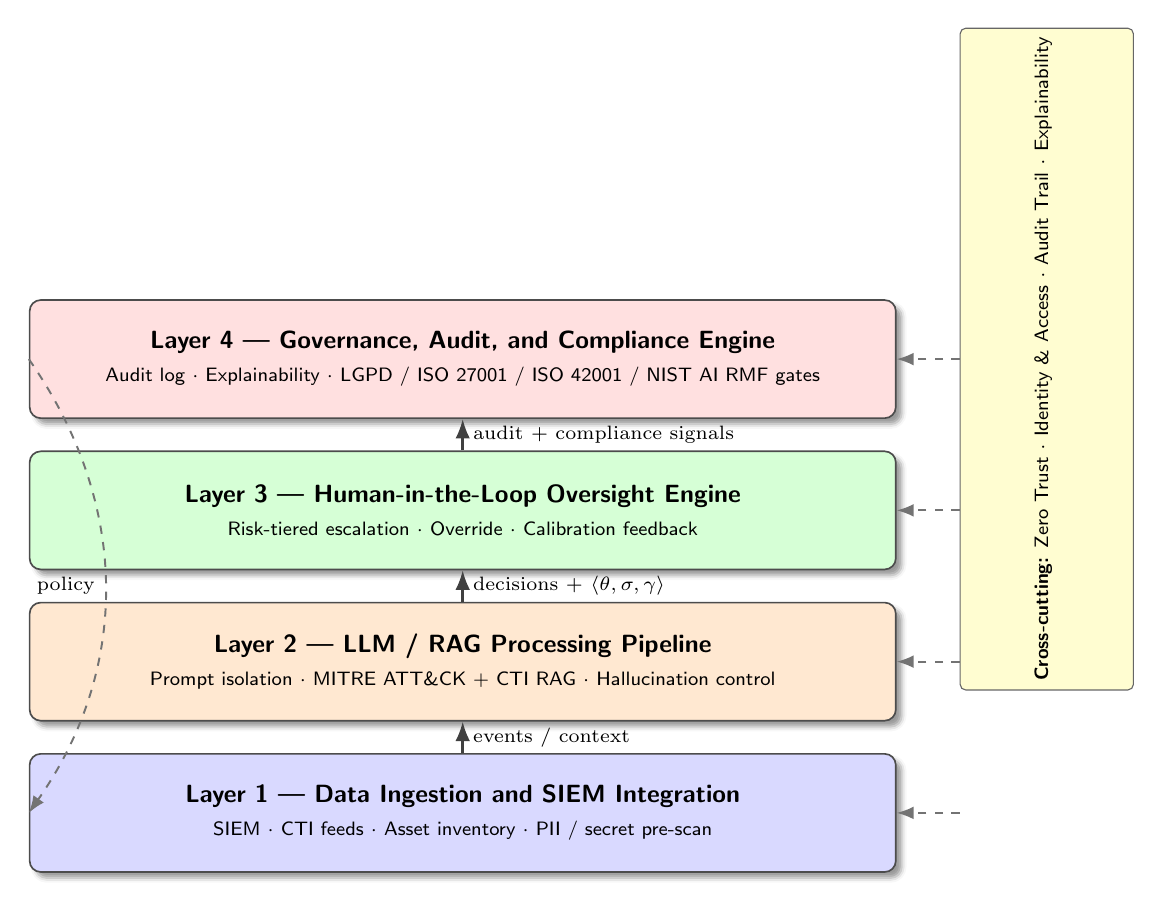
\begin{tikzpicture}[node distance=4mm]
  \node[L4] (L4) {%
    \textbf{Layer 4 — Governance, Audit, and Compliance Engine}\\[1pt]
    \scriptsize Audit log $\cdot$ Explainability $\cdot$ LGPD / ISO 27001 / ISO 42001 / NIST AI RMF gates};
  \node[L3, below=of L4] (L3) {%
    \textbf{Layer 3 — Human-in-the-Loop Oversight Engine}\\[1pt]
    \scriptsize Risk-tiered escalation $\cdot$ Override $\cdot$ Calibration feedback};
  \node[L2, below=of L3] (L2) {%
    \textbf{Layer 2 — LLM / RAG Processing Pipeline}\\[1pt]
    \scriptsize Prompt isolation $\cdot$ MITRE ATT\&CK + CTI RAG $\cdot$ Hallucination control};
  \node[L1, below=of L2] (L1) {%
    \textbf{Layer 1 — Data Ingestion and SIEM Integration}\\[1pt]
    \scriptsize SIEM $\cdot$ CTI feeds $\cdot$ Asset inventory $\cdot$ PII / secret pre-scan};

  % Cross-cutting concerns on the right
  \node[side, right=8mm of L4.east,
        anchor=west, minimum height=8.0cm] (cross) {%
    \rotatebox{90}{\textbf{Cross-cutting:} Zero Trust $\cdot$ Identity \& Access $\cdot$ Audit Trail $\cdot$ Explainability}
  };
  \draw[flowdash] (cross.west|-L4.east) -- (L4.east);
  \draw[flowdash] (cross.west|-L3.east) -- (L3.east);
  \draw[flowdash] (cross.west|-L2.east) -- (L2.east);
  \draw[flowdash] (cross.west|-L1.east) -- (L1.east);

  % Flows between layers
  \draw[flow] (L1.north) -- (L2.south) node[midway, right, font=\scriptsize] {events / context};
  \draw[flow] (L2.north) -- (L3.south) node[midway, right, font=\scriptsize] {decisions + $\langle\theta,\sigma,\gamma\rangle$};
  \draw[flow] (L3.north) -- (L4.south) node[midway, right, font=\scriptsize] {audit + compliance signals};
  \draw[flowdash] (L4.west)+(0,0) to[bend left=35] node[left, font=\scriptsize] {policy} (L1.west);

\end{tikzpicture}
% Caption (for manuscript):
% Figure 1. SHIELD-AI four-layer architecture. Layers are governed top-down by
% standards-aligned policy (L4 → L1) and produce upward flows of events,
% decisions with reliability triples ⟨θ, σ, γ⟩, and audit signals. Cross-cutting
% concerns (Zero Trust, Identity & Access, Audit Trail, Explainability) operate
% across all layers.

% =====================================================================
% F2 — Offensive--Defensive AI Cycle in Cybersecurity
% =====================================================================
\newpage
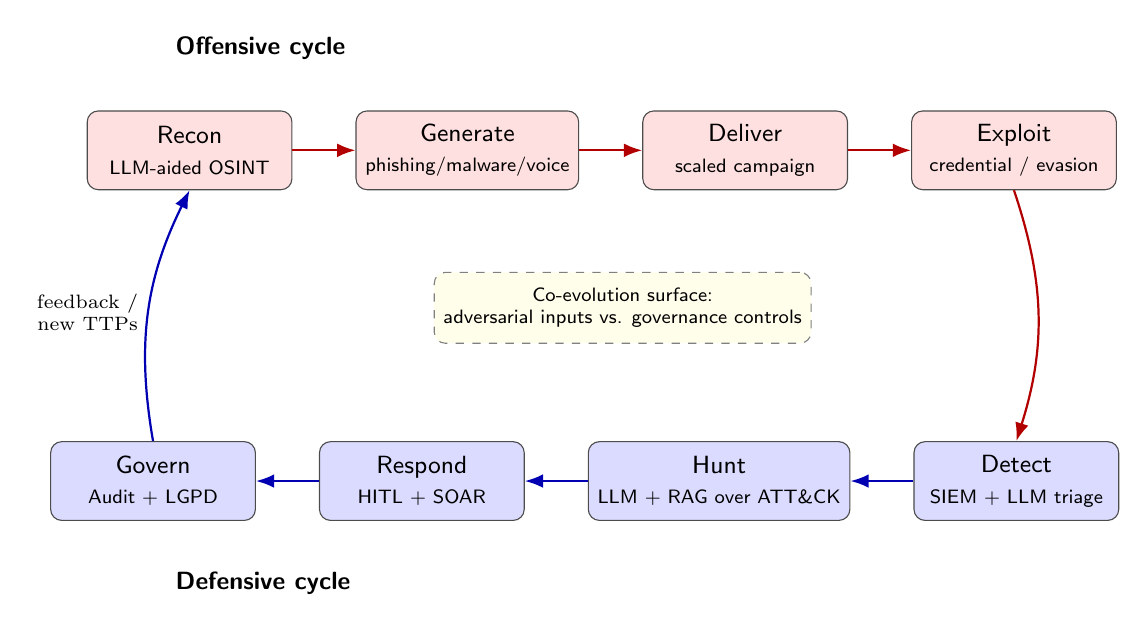
\begin{tikzpicture}[
    node distance=8mm,
    stage/.style={rectangle, rounded corners=4pt, draw=black!70,
                  minimum width=2.6cm, minimum height=1.0cm,
                  align=center, font=\small\sffamily},
    off/.style={stage, fill=red!12},
    def/.style={stage, fill=blue!14},
    cycle/.style={-Latex, line width=0.8pt}
]
  % Offensive stages (top half)
  \node[off] (recon) at (0,3) {Recon\\\scriptsize LLM-aided OSINT};
  \node[off, right=of recon] (gen) {Generate\\\scriptsize phishing/malware/voice};
  \node[off, right=of gen] (deliver) {Deliver\\\scriptsize scaled campaign};
  \node[off, right=of deliver] (exploit) {Exploit\\\scriptsize credential / evasion};

  % Defensive stages (bottom half)
  \node[def] (detect) at (10.5,-1.2) {Detect\\\scriptsize SIEM + LLM triage};
  \node[def, left=of detect] (hunt) {Hunt\\\scriptsize LLM + RAG over ATT\&CK};
  \node[def, left=of hunt] (resp) {Respond\\\scriptsize HITL + SOAR};
  \node[def, left=of resp] (gov) {Govern\\\scriptsize Audit + LGPD};

  % Connecting arrows
  \draw[cycle, draw=red!70!black] (recon) -- (gen);
  \draw[cycle, draw=red!70!black] (gen) -- (deliver);
  \draw[cycle, draw=red!70!black] (deliver) -- (exploit);
  \draw[cycle, draw=red!70!black] (exploit.south) to[bend left=18] (detect.north);

  \draw[cycle, draw=blue!70!black] (detect) -- (hunt);
  \draw[cycle, draw=blue!70!black] (hunt) -- (resp);
  \draw[cycle, draw=blue!70!black] (resp) -- (gov);
  \draw[cycle, draw=blue!70!black] (gov.north) to[bend left=18]
     node[left, font=\scriptsize, align=center] {feedback /\\new TTPs} (recon.south);

  % Central "AI-vs-AI" annotation
  \node[draw=black!50, dashed, rounded corners=4pt,
        fill=yellow!8, font=\scriptsize\sffamily, align=center,
        minimum width=4cm, minimum height=0.9cm] (core) at (5.5,1.0)
        {Co-evolution surface:\\ adversarial inputs vs. governance controls};

  \node[font=\bfseries\sffamily\small, anchor=west] at (-0.3, 4.3) {Offensive cycle};
  \node[font=\bfseries\sffamily\small, anchor=west] at (-0.3, -2.5) {Defensive cycle};

\end{tikzpicture}
% Caption:
% Figure 2. Offensive--defensive AI co-evolution. Generative AI accelerates
% adversary operations (top); defensive AI must accelerate detection, hunting,
% response, and governance (bottom). The two cycles share a co-evolution
% surface, including prompt-injection and tool-poisoning vectors against the
% defensive AI itself.

% =====================================================================
% F3 — SOC Pipeline (Data Flow Detail)
% =====================================================================
\newpage
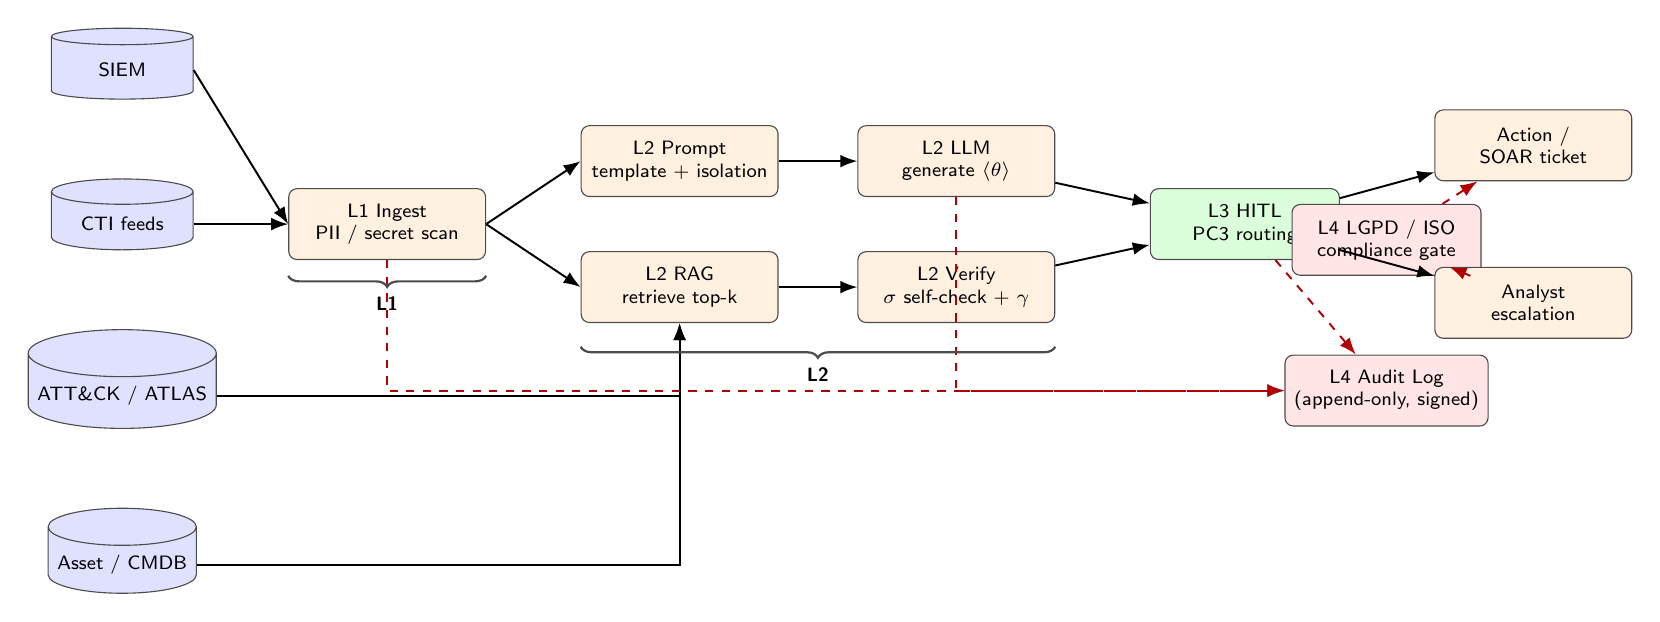
\begin{tikzpicture}[node distance=10mm,
    src/.style={cylinder, shape border rotate=90, aspect=0.25,
                draw=black!70, fill=blue!12, minimum height=0.9cm,
                minimum width=1.8cm, font=\scriptsize\sffamily, align=center},
    blk/.style={rectangle, rounded corners=3pt, draw=black!70,
                fill=orange!12, minimum width=2.5cm, minimum height=0.9cm,
                font=\scriptsize\sffamily, align=center},
    eng/.style={rectangle, rounded corners=3pt, draw=black!70,
                fill=green!14, minimum width=2.4cm, minimum height=0.9cm,
                font=\scriptsize\sffamily, align=center},
    gov/.style={rectangle, rounded corners=3pt, draw=black!70,
                fill=red!10, minimum width=2.4cm, minimum height=0.9cm,
                font=\scriptsize\sffamily, align=center},
    arr/.style={-Latex, line width=0.7pt}
]
  % Sources (left column)
  \node[src] (siem) {SIEM};
  \node[src, below=of siem] (cti)  {CTI feeds};
  \node[src, below=of cti]  (attck){ATT\&CK / ATLAS};
  \node[src, below=of attck] (cmdb){Asset / CMDB};

  % L1
  \node[blk, right=12mm of cti] (ingest) {L1 Ingest\\PII / secret scan};

  % L2 LLM/RAG pipeline
  \node[blk, right=12mm of ingest, yshift=8mm]  (prompt) {L2 Prompt\\template + isolation};
  \node[blk, right=12mm of ingest, yshift=-8mm] (rag)    {L2 RAG\\retrieve top-k};
  \node[blk, right=of prompt] (llm) {L2 LLM\\generate $\langle\theta\rangle$};
  \node[blk, right=of rag]    (check){L2 Verify\\$\sigma$ self-check + $\gamma$};

  % L3 HITL
  \node[eng, right=12mm of llm, yshift=-8mm] (hitl) {L3 HITL\\PC3 routing};

  % L4 Governance
  \node[gov, below=12mm of hitl, xshift=18mm] (audit) {L4 Audit Log\\(append-only, signed)};
  \node[gov, above=of audit] (compl) {L4 LGPD / ISO\\ compliance gate};

  % Final outputs
  \node[blk, right=12mm of hitl, yshift=10mm] (action) {Action /\\SOAR ticket};
  \node[blk, right=12mm of hitl, yshift=-10mm](escal)  {Analyst\\escalation};

  % Arrows
  \draw[arr] (siem.east)  -- (ingest.west);
  \draw[arr] (cti.east)   -- (ingest.west);
  \draw[arr] (attck.east) -| (rag.south);
  \draw[arr] (cmdb.east)  -| (rag.south);
  \draw[arr] (ingest.east) -- (prompt.west);
  \draw[arr] (ingest.east) -- (rag.west);
  \draw[arr] (prompt) -- (llm);
  \draw[arr] (rag) -- (check);
  \draw[arr] (llm) -- (hitl);
  \draw[arr] (check) -- (hitl);
  \draw[arr] (hitl) -- (action);
  \draw[arr] (hitl) -- (escal);

  % L4 governance arrows (dashed, two-way)
  \draw[arr, dashed, draw=red!70!black] (hitl) -- (audit);
  \draw[arr, dashed, draw=red!70!black] (llm) |- (audit);
  \draw[arr, dashed, draw=red!70!black] (ingest) |- (audit);
  \draw[arr, dashed, draw=red!70!black] (compl) -- (action);
  \draw[arr, dashed, draw=red!70!black] (compl) -- (escal);

  % Layer brackets
  \draw[decorate, decoration={brace, amplitude=4pt, mirror},
        line width=0.8pt, draw=black!70]
       ($(ingest.south west)+(0,-0.2)$) -- ($(ingest.south east)+(0,-0.2)$)
       node[midway, below=4pt, font=\bfseries\scriptsize\sffamily] {L1};
  \draw[decorate, decoration={brace, amplitude=4pt, mirror},
        line width=0.8pt, draw=black!70]
       ($(rag.south west)+(0,-0.3)$) -- ($(check.south east)+(0,-0.3)$)
       node[midway, below=4pt, font=\bfseries\scriptsize\sffamily] {L2};
\end{tikzpicture}
% Caption:
% Figure 3. SHIELD-AI SOC pipeline detail. L1 ingests events from SIEM, CTI,
% and asset inventory with PII pre-scanning. L2 isolates prompt and data, runs
% RAG over MITRE ATT&CK/ATLAS, and computes the reliability triple ⟨θ, σ, γ⟩.
% L3 routes outputs through PC3 (auto / HITL / reject). L4 records every step
% in an append-only audit log and gates outgoing actions against LGPD and ISO
% requirements.

% =====================================================================
% F4 — Governance and Audit Model
% =====================================================================
\newpage
\begin{tikzpicture}[
    node distance=7mm,
    obj/.style={rectangle, rounded corners=3pt, draw=black!70,
                minimum width=3.2cm, minimum height=0.9cm,
                font=\scriptsize\sffamily, align=center},
    invar/.style={obj, fill=red!12},
    ctrl/.style={obj, fill=orange!14},
    std/.style={obj, fill=blue!12},
    arr/.style={-Latex, line width=0.7pt}
]
  % Center: audit invariant
  \node[invar, minimum width=5.6cm, minimum height=1.2cm] (A)
       {\textbf{Audit Invariant 𝓐} \\
        $\langle$input, prompt, retrieved, output, $\theta,\sigma,\gamma$, route, analyst, ts$\rangle$};

  % Controls feeding into 𝓐
  \node[ctrl, above left=of A] (c1) {Input sanitization};
  \node[ctrl, above=of A]      (c2) {Self-check + RAG verification};
  \node[ctrl, above right=of A](c3) {HITL routing};
  \node[ctrl, below left=of A] (c4) {Tool allowlist};
  \node[ctrl, below=of A]      (c5) {LGPD / PII gate};
  \node[ctrl, below right=of A](c6) {Identity / Zero-Trust};

  \foreach \c in {c1,c2,c3,c4,c5,c6}{
    \draw[arr] (\c) -- (A);
  }

  % Standards arrayed on right (𝓜 mapping) — extra horizontal space avoids label overlap
  \node[std, right=42mm of A.east, yshift=22mm] (s1) {MITRE ATT\&CK / ATLAS};
  \node[std, right=42mm of A.east, yshift= 8mm] (s2) {NIST CSF 2.0 / AI RMF};
  \node[std, right=42mm of A.east, yshift=-6mm] (s3) {OWASP LLM \& Agentic};
  \node[std, right=42mm of A.east, yshift=-20mm](s4) {ISO 27001 / 42001 / LGPD};

  % Mapping 𝓜 arrows from controls to standards — route around control labels
  \draw[arr, draw=blue!60!black, dashed] (c3.east) -- ++(0.6,0) |- (s1.west);
  \draw[arr, draw=blue!60!black, dashed] (c2.north east) -- ++(0.4,0) |- (s1.west);
  \draw[arr, draw=blue!60!black, dashed] (c1.east) -- ++(0.6,0) |- (s3.west);
  \draw[arr, draw=blue!60!black, dashed] (c5.east) -- ++(0.6,0) |- (s4.west);
  \draw[arr, draw=blue!60!black, dashed] (c6.east) -- ++(0.6,0) |- (s2.west);

  % Property output
  \node[obj, fill=green!14, left=18mm of A.west] (P) {Properties 𝓟\\(P1--P7)};
  \draw[arr, draw=green!60!black] (A) -- (P);

  \node[font=\itshape\scriptsize\sffamily, anchor=north, text width=4cm]
    at ($(P.south)+(0,-1mm)$)
    {Audit-complete $\cdot$ CGS-monotone $\cdot$ Compliance-preserving $\cdot$ Policy-derivable HITL};

\end{tikzpicture}
% Caption:
% Figure 4. Governance and audit model. Controls (orange) emit audit tuples
% into the invariant 𝓐 (red center). The mapping 𝓜 (dashed blue) routes each
% control to its corresponding external standards. Properties 𝓟 (green, left)
% are guaranteed by construction (see Lemmas 1--2 and Theorems 1--3).

% =====================================================================
% F5 — Research Method Flow (DSR + SLM + Scenario Evaluation)
% =====================================================================
\newpage
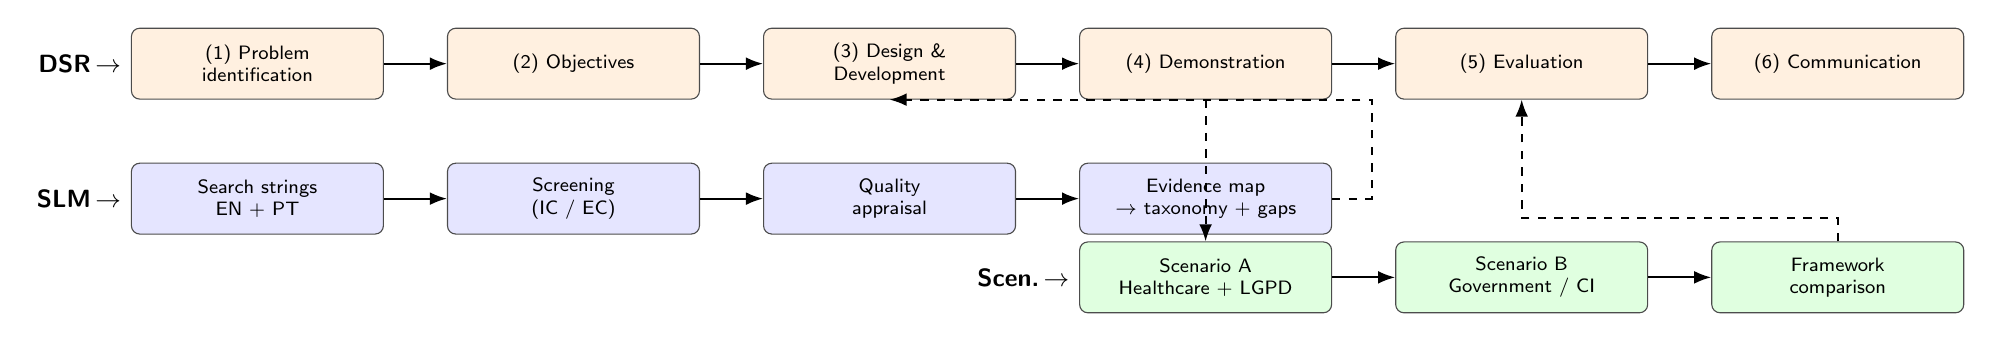
\begin{tikzpicture}[
    node distance=8mm,
    stepbox/.style={rectangle, rounded corners=3pt, draw=black!70,
                 minimum width=3.2cm, minimum height=0.9cm,
                 font=\scriptsize\sffamily, align=center},
    slm/.style={stepbox, fill=blue!10},
    dsr/.style={stepbox, fill=orange!12},
    eval/.style={stepbox, fill=green!12},
    arr/.style={-Latex, line width=0.7pt}
]
  % DSR (top row)
  \node[dsr] (p1) {(1) Problem\\identification};
  \node[dsr, right=of p1] (p2) {(2) Objectives};
  \node[dsr, right=of p2] (p3) {(3) Design \&\\Development};
  \node[dsr, right=of p3] (p4) {(4) Demonstration};
  \node[dsr, right=of p4] (p5) {(5) Evaluation};
  \node[dsr, right=of p5] (p6) {(6) Communication};

  \foreach \a/\b in {p1/p2, p2/p3, p3/p4, p4/p5, p5/p6}{
    \draw[arr] (\a) -- (\b);
  }

  % SLM (below, anchored to p1, p2)
  \node[slm, below=of p1] (s1) {Search strings\\EN + PT};
  \node[slm, right=of s1] (s2) {Screening\\(IC / EC)};
  \node[slm, right=of s2] (s3) {Quality\\appraisal};
  \node[slm, right=of s3] (s4) {Evidence map\\$\rightarrow$ taxonomy + gaps};
  \draw[arr] (s1) -- (s2);
  \draw[arr] (s2) -- (s3);
  \draw[arr] (s3) -- (s4);
  \draw[arr, dashed] (s4.east) -- ++(0.5,0) |- (p3.south);

  % Scenarios (below, anchored to p4, p5)
  \node[eval, below=18mm of p4] (e1) {Scenario A\\Healthcare + LGPD};
  \node[eval, right=of e1]      (e2) {Scenario B\\Government / CI};
  \node[eval, right=of e2]      (e3) {Framework\\comparison};
  \draw[arr] (e1) -- (e2);
  \draw[arr] (e2) -- (e3);
  \draw[arr, dashed] (p4.south) -- ++(0,-0.3) -- (e1.north);
  \draw[arr, dashed] (e3.north) -- ++(0,0.3) -| (p5.south);

  % Labels
  \node[font=\bfseries\small\sffamily, anchor=east] at (p1.west) {DSR\,$\rightarrow$};
  \node[font=\bfseries\small\sffamily, anchor=east] at (s1.west) {SLM\,$\rightarrow$};
  \node[font=\bfseries\small\sffamily, anchor=east] at (e1.west) {Scen.\,$\rightarrow$};
\end{tikzpicture}
% Caption:
% Figure 5. Research method flow. The Design Science Research process (Peffers
% DSRM, top row) is fed by a Systematic Literature Mapping (middle) and
% evaluated by structured scenario analyses (bottom).

\end{document}

%
% Each figure is wrapped in a \begin{figure} block so it can be moved into the
% manuscript at Stage 5 with minor adjustments (positioning/captions).

\documentclass[tikz,border=8pt]{standalone}
\usepackage[utf8]{inputenc}
\usepackage[T1]{fontenc}
\usepackage{tikz}
\usepackage{amsmath,amssymb}
\usetikzlibrary{shapes.geometric,arrows.meta,positioning,fit,backgrounds,
                calc,decorations.pathreplacing,decorations.pathmorphing,
                shadows.blur,patterns}

% ===== Reusable styles =====
\tikzset{
  layer/.style={
    rectangle, rounded corners=4pt, draw=black!70, line width=0.6pt,
    minimum width=11cm, minimum height=1.5cm,
    align=center, font=\small\sffamily, blur shadow={shadow blur steps=3}
  },
  L1/.style={layer, fill=blue!15},
  L2/.style={layer, fill=orange!18},
  L3/.style={layer, fill=green!16},
  L4/.style={layer, fill=red!12},
  flow/.style={-Latex, line width=0.9pt, draw=black!75},
  flowdash/.style={-Latex, line width=0.7pt, draw=black!55, dashed},
  comp/.style={rectangle, rounded corners=3pt, draw=black!65,
               fill=white, minimum width=2.4cm, minimum height=0.7cm,
               font=\footnotesize\sffamily, align=center},
  side/.style={rectangle, rounded corners=2pt, draw=black!60, fill=yellow!18,
               font=\scriptsize\sffamily, align=center,
               minimum width=2.2cm, minimum height=0.55cm},
  label/.style={font=\bfseries\sffamily\small, anchor=west},
  axislbl/.style={font=\footnotesize\itshape, anchor=west}
}

\begin{document}

% =====================================================================
% F1 — SHIELD-AI Four-Layer Architecture
% =====================================================================
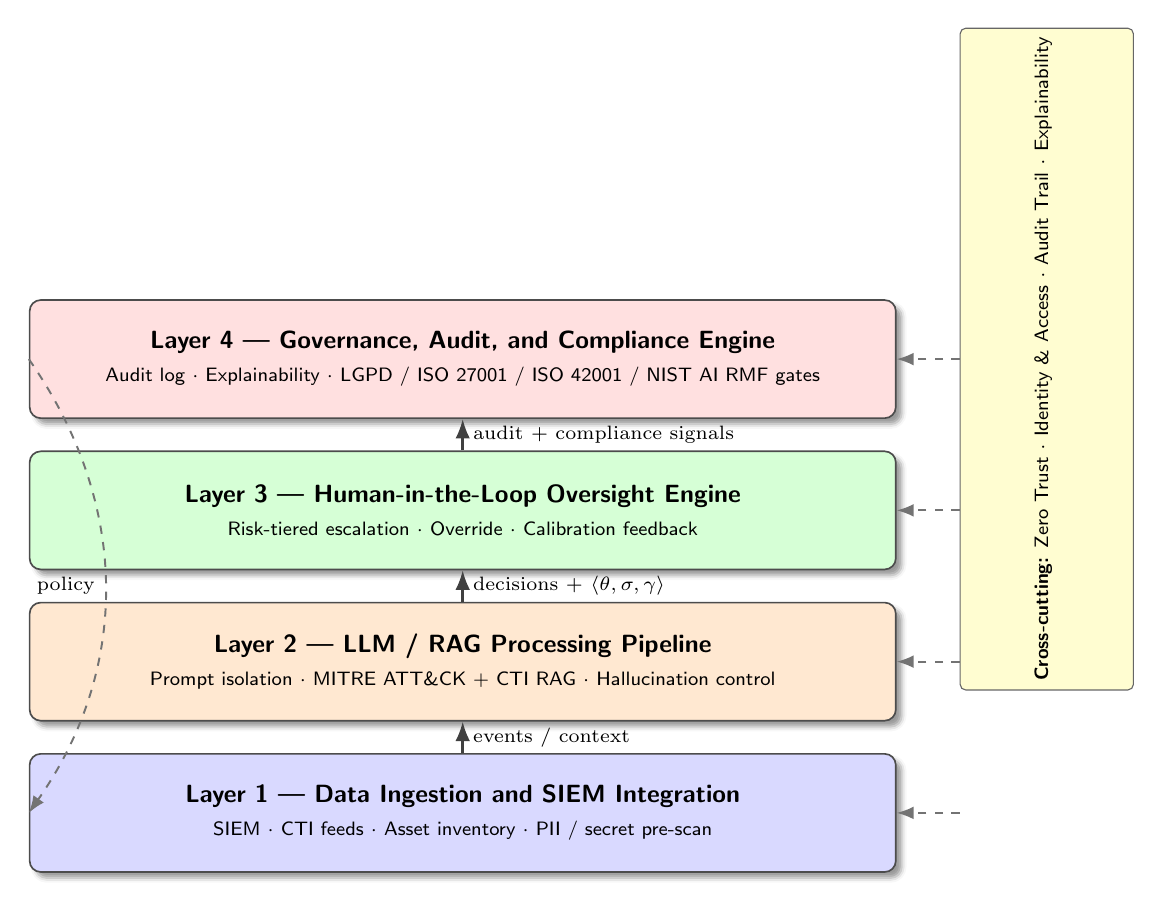
\begin{tikzpicture}[node distance=4mm]
  \node[L4] (L4) {%
    \textbf{Layer 4 — Governance, Audit, and Compliance Engine}\\[1pt]
    \scriptsize Audit log $\cdot$ Explainability $\cdot$ LGPD / ISO 27001 / ISO 42001 / NIST AI RMF gates};
  \node[L3, below=of L4] (L3) {%
    \textbf{Layer 3 — Human-in-the-Loop Oversight Engine}\\[1pt]
    \scriptsize Risk-tiered escalation $\cdot$ Override $\cdot$ Calibration feedback};
  \node[L2, below=of L3] (L2) {%
    \textbf{Layer 2 — LLM / RAG Processing Pipeline}\\[1pt]
    \scriptsize Prompt isolation $\cdot$ MITRE ATT\&CK + CTI RAG $\cdot$ Hallucination control};
  \node[L1, below=of L2] (L1) {%
    \textbf{Layer 1 — Data Ingestion and SIEM Integration}\\[1pt]
    \scriptsize SIEM $\cdot$ CTI feeds $\cdot$ Asset inventory $\cdot$ PII / secret pre-scan};

  % Cross-cutting concerns on the right
  \node[side, right=8mm of L4.east,
        anchor=west, minimum height=8.0cm] (cross) {%
    \rotatebox{90}{\textbf{Cross-cutting:} Zero Trust $\cdot$ Identity \& Access $\cdot$ Audit Trail $\cdot$ Explainability}
  };
  \draw[flowdash] (cross.west|-L4.east) -- (L4.east);
  \draw[flowdash] (cross.west|-L3.east) -- (L3.east);
  \draw[flowdash] (cross.west|-L2.east) -- (L2.east);
  \draw[flowdash] (cross.west|-L1.east) -- (L1.east);

  % Flows between layers
  \draw[flow] (L1.north) -- (L2.south) node[midway, right, font=\scriptsize] {events / context};
  \draw[flow] (L2.north) -- (L3.south) node[midway, right, font=\scriptsize] {decisions + $\langle\theta,\sigma,\gamma\rangle$};
  \draw[flow] (L3.north) -- (L4.south) node[midway, right, font=\scriptsize] {audit + compliance signals};
  \draw[flowdash] (L4.west)+(0,0) to[bend left=35] node[left, font=\scriptsize] {policy} (L1.west);

\end{tikzpicture}
% Caption (for manuscript):
% Figure 1. SHIELD-AI four-layer architecture. Layers are governed top-down by
% standards-aligned policy (L4 → L1) and produce upward flows of events,
% decisions with reliability triples ⟨θ, σ, γ⟩, and audit signals. Cross-cutting
% concerns (Zero Trust, Identity & Access, Audit Trail, Explainability) operate
% across all layers.

% =====================================================================
% F2 — Offensive--Defensive AI Cycle in Cybersecurity
% =====================================================================
\newpage
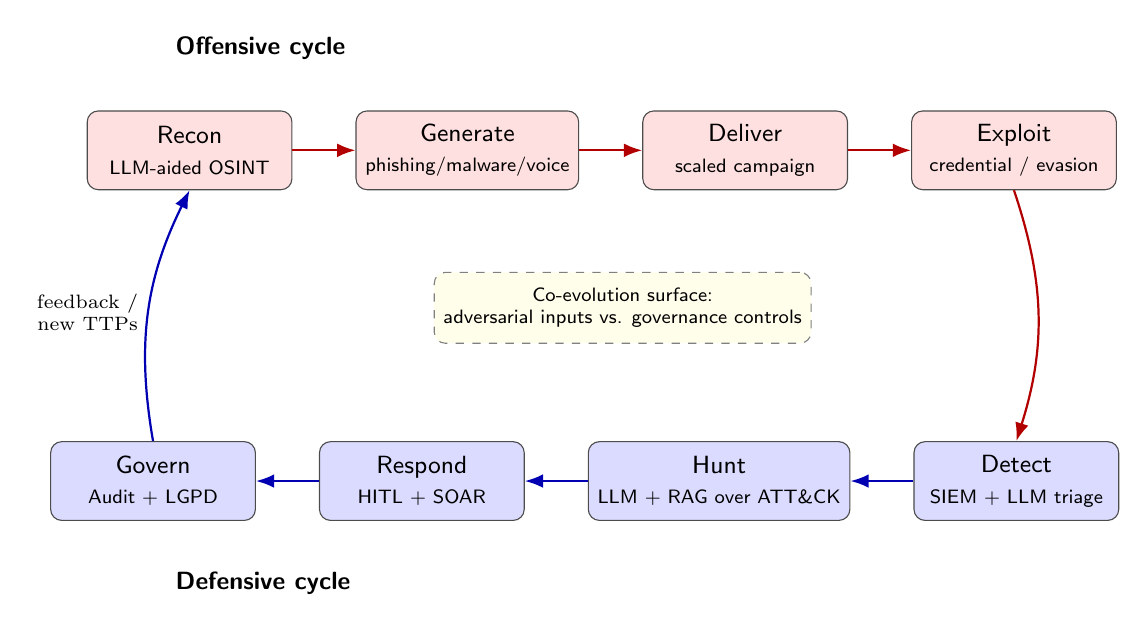
\begin{tikzpicture}[
    node distance=8mm,
    stage/.style={rectangle, rounded corners=4pt, draw=black!70,
                  minimum width=2.6cm, minimum height=1.0cm,
                  align=center, font=\small\sffamily},
    off/.style={stage, fill=red!12},
    def/.style={stage, fill=blue!14},
    cycle/.style={-Latex, line width=0.8pt}
]
  % Offensive stages (top half)
  \node[off] (recon) at (0,3) {Recon\\\scriptsize LLM-aided OSINT};
  \node[off, right=of recon] (gen) {Generate\\\scriptsize phishing/malware/voice};
  \node[off, right=of gen] (deliver) {Deliver\\\scriptsize scaled campaign};
  \node[off, right=of deliver] (exploit) {Exploit\\\scriptsize credential / evasion};

  % Defensive stages (bottom half)
  \node[def] (detect) at (10.5,-1.2) {Detect\\\scriptsize SIEM + LLM triage};
  \node[def, left=of detect] (hunt) {Hunt\\\scriptsize LLM + RAG over ATT\&CK};
  \node[def, left=of hunt] (resp) {Respond\\\scriptsize HITL + SOAR};
  \node[def, left=of resp] (gov) {Govern\\\scriptsize Audit + LGPD};

  % Connecting arrows
  \draw[cycle, draw=red!70!black] (recon) -- (gen);
  \draw[cycle, draw=red!70!black] (gen) -- (deliver);
  \draw[cycle, draw=red!70!black] (deliver) -- (exploit);
  \draw[cycle, draw=red!70!black] (exploit.south) to[bend left=18] (detect.north);

  \draw[cycle, draw=blue!70!black] (detect) -- (hunt);
  \draw[cycle, draw=blue!70!black] (hunt) -- (resp);
  \draw[cycle, draw=blue!70!black] (resp) -- (gov);
  \draw[cycle, draw=blue!70!black] (gov.north) to[bend left=18]
     node[left, font=\scriptsize, align=center] {feedback /\\new TTPs} (recon.south);

  % Central "AI-vs-AI" annotation
  \node[draw=black!50, dashed, rounded corners=4pt,
        fill=yellow!8, font=\scriptsize\sffamily, align=center,
        minimum width=4cm, minimum height=0.9cm] (core) at (5.5,1.0)
        {Co-evolution surface:\\ adversarial inputs vs. governance controls};

  \node[font=\bfseries\sffamily\small, anchor=west] at (-0.3, 4.3) {Offensive cycle};
  \node[font=\bfseries\sffamily\small, anchor=west] at (-0.3, -2.5) {Defensive cycle};

\end{tikzpicture}
% Caption:
% Figure 2. Offensive--defensive AI co-evolution. Generative AI accelerates
% adversary operations (top); defensive AI must accelerate detection, hunting,
% response, and governance (bottom). The two cycles share a co-evolution
% surface, including prompt-injection and tool-poisoning vectors against the
% defensive AI itself.

% =====================================================================
% F3 — SOC Pipeline (Data Flow Detail)
% =====================================================================
\newpage
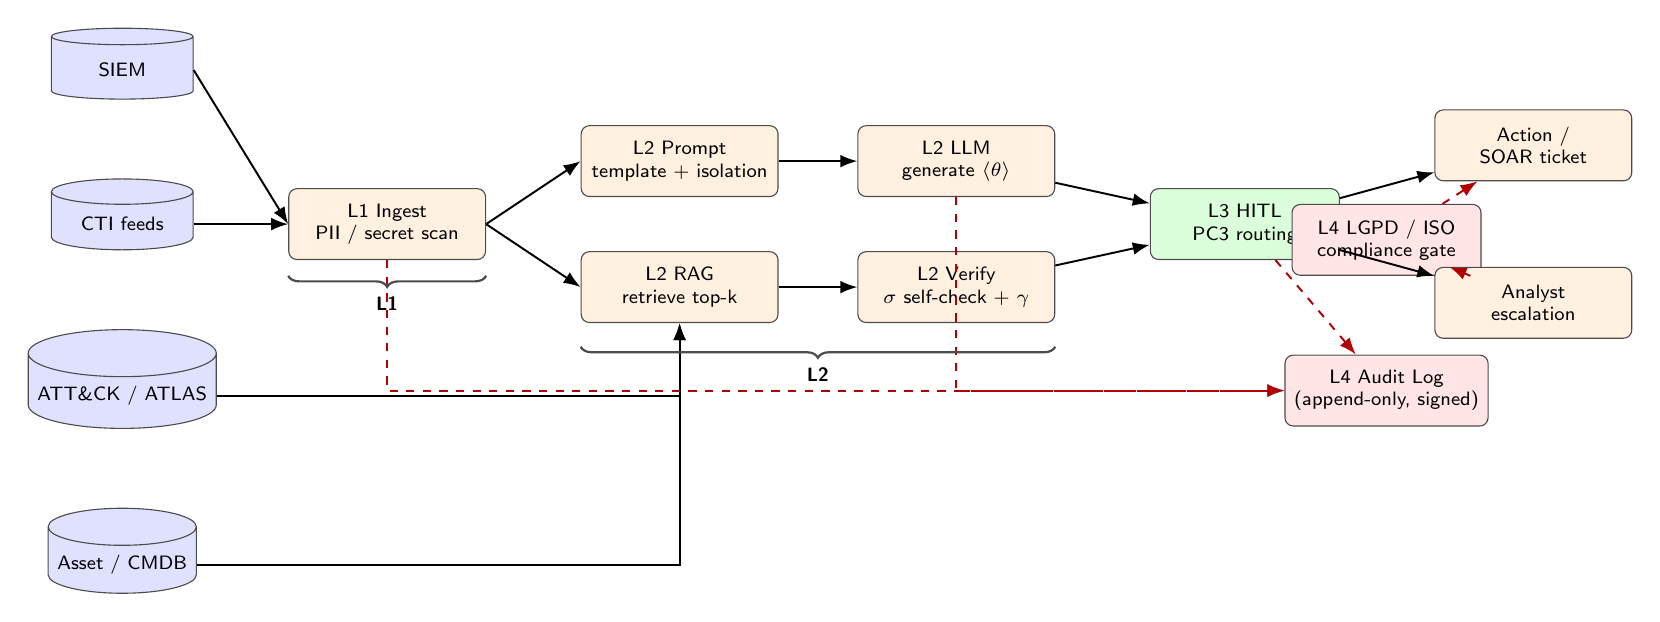
\begin{tikzpicture}[node distance=10mm,
    src/.style={cylinder, shape border rotate=90, aspect=0.25,
                draw=black!70, fill=blue!12, minimum height=0.9cm,
                minimum width=1.8cm, font=\scriptsize\sffamily, align=center},
    blk/.style={rectangle, rounded corners=3pt, draw=black!70,
                fill=orange!12, minimum width=2.5cm, minimum height=0.9cm,
                font=\scriptsize\sffamily, align=center},
    eng/.style={rectangle, rounded corners=3pt, draw=black!70,
                fill=green!14, minimum width=2.4cm, minimum height=0.9cm,
                font=\scriptsize\sffamily, align=center},
    gov/.style={rectangle, rounded corners=3pt, draw=black!70,
                fill=red!10, minimum width=2.4cm, minimum height=0.9cm,
                font=\scriptsize\sffamily, align=center},
    arr/.style={-Latex, line width=0.7pt}
]
  % Sources (left column)
  \node[src] (siem) {SIEM};
  \node[src, below=of siem] (cti)  {CTI feeds};
  \node[src, below=of cti]  (attck){ATT\&CK / ATLAS};
  \node[src, below=of attck] (cmdb){Asset / CMDB};

  % L1
  \node[blk, right=12mm of cti] (ingest) {L1 Ingest\\PII / secret scan};

  % L2 LLM/RAG pipeline
  \node[blk, right=12mm of ingest, yshift=8mm]  (prompt) {L2 Prompt\\template + isolation};
  \node[blk, right=12mm of ingest, yshift=-8mm] (rag)    {L2 RAG\\retrieve top-k};
  \node[blk, right=of prompt] (llm) {L2 LLM\\generate $\langle\theta\rangle$};
  \node[blk, right=of rag]    (check){L2 Verify\\$\sigma$ self-check + $\gamma$};

  % L3 HITL
  \node[eng, right=12mm of llm, yshift=-8mm] (hitl) {L3 HITL\\PC3 routing};

  % L4 Governance
  \node[gov, below=12mm of hitl, xshift=18mm] (audit) {L4 Audit Log\\(append-only, signed)};
  \node[gov, above=of audit] (compl) {L4 LGPD / ISO\\ compliance gate};

  % Final outputs
  \node[blk, right=12mm of hitl, yshift=10mm] (action) {Action /\\SOAR ticket};
  \node[blk, right=12mm of hitl, yshift=-10mm](escal)  {Analyst\\escalation};

  % Arrows
  \draw[arr] (siem.east)  -- (ingest.west);
  \draw[arr] (cti.east)   -- (ingest.west);
  \draw[arr] (attck.east) -| (rag.south);
  \draw[arr] (cmdb.east)  -| (rag.south);
  \draw[arr] (ingest.east) -- (prompt.west);
  \draw[arr] (ingest.east) -- (rag.west);
  \draw[arr] (prompt) -- (llm);
  \draw[arr] (rag) -- (check);
  \draw[arr] (llm) -- (hitl);
  \draw[arr] (check) -- (hitl);
  \draw[arr] (hitl) -- (action);
  \draw[arr] (hitl) -- (escal);

  % L4 governance arrows (dashed, two-way)
  \draw[arr, dashed, draw=red!70!black] (hitl) -- (audit);
  \draw[arr, dashed, draw=red!70!black] (llm) |- (audit);
  \draw[arr, dashed, draw=red!70!black] (ingest) |- (audit);
  \draw[arr, dashed, draw=red!70!black] (compl) -- (action);
  \draw[arr, dashed, draw=red!70!black] (compl) -- (escal);

  % Layer brackets
  \draw[decorate, decoration={brace, amplitude=4pt, mirror},
        line width=0.8pt, draw=black!70]
       ($(ingest.south west)+(0,-0.2)$) -- ($(ingest.south east)+(0,-0.2)$)
       node[midway, below=4pt, font=\bfseries\scriptsize\sffamily] {L1};
  \draw[decorate, decoration={brace, amplitude=4pt, mirror},
        line width=0.8pt, draw=black!70]
       ($(rag.south west)+(0,-0.3)$) -- ($(check.south east)+(0,-0.3)$)
       node[midway, below=4pt, font=\bfseries\scriptsize\sffamily] {L2};
\end{tikzpicture}
% Caption:
% Figure 3. SHIELD-AI SOC pipeline detail. L1 ingests events from SIEM, CTI,
% and asset inventory with PII pre-scanning. L2 isolates prompt and data, runs
% RAG over MITRE ATT&CK/ATLAS, and computes the reliability triple ⟨θ, σ, γ⟩.
% L3 routes outputs through PC3 (auto / HITL / reject). L4 records every step
% in an append-only audit log and gates outgoing actions against LGPD and ISO
% requirements.

% =====================================================================
% F4 — Governance and Audit Model
% =====================================================================
\newpage
\begin{tikzpicture}[
    node distance=7mm,
    obj/.style={rectangle, rounded corners=3pt, draw=black!70,
                minimum width=3.2cm, minimum height=0.9cm,
                font=\scriptsize\sffamily, align=center},
    invar/.style={obj, fill=red!12},
    ctrl/.style={obj, fill=orange!14},
    std/.style={obj, fill=blue!12},
    arr/.style={-Latex, line width=0.7pt}
]
  % Center: audit invariant
  \node[invar, minimum width=5.6cm, minimum height=1.2cm] (A)
       {\textbf{Audit Invariant 𝓐} \\
        $\langle$input, prompt, retrieved, output, $\theta,\sigma,\gamma$, route, analyst, ts$\rangle$};

  % Controls feeding into 𝓐
  \node[ctrl, above left=of A] (c1) {Input sanitization};
  \node[ctrl, above=of A]      (c2) {Self-check + RAG verification};
  \node[ctrl, above right=of A](c3) {HITL routing};
  \node[ctrl, below left=of A] (c4) {Tool allowlist};
  \node[ctrl, below=of A]      (c5) {LGPD / PII gate};
  \node[ctrl, below right=of A](c6) {Identity / Zero-Trust};

  \foreach \c in {c1,c2,c3,c4,c5,c6}{
    \draw[arr] (\c) -- (A);
  }

  % Standards arrayed on right (𝓜 mapping) — extra horizontal space avoids label overlap
  \node[std, right=42mm of A.east, yshift=22mm] (s1) {MITRE ATT\&CK / ATLAS};
  \node[std, right=42mm of A.east, yshift= 8mm] (s2) {NIST CSF 2.0 / AI RMF};
  \node[std, right=42mm of A.east, yshift=-6mm] (s3) {OWASP LLM \& Agentic};
  \node[std, right=42mm of A.east, yshift=-20mm](s4) {ISO 27001 / 42001 / LGPD};

  % Mapping 𝓜 arrows from controls to standards — route around control labels
  \draw[arr, draw=blue!60!black, dashed] (c3.east) -- ++(0.6,0) |- (s1.west);
  \draw[arr, draw=blue!60!black, dashed] (c2.north east) -- ++(0.4,0) |- (s1.west);
  \draw[arr, draw=blue!60!black, dashed] (c1.east) -- ++(0.6,0) |- (s3.west);
  \draw[arr, draw=blue!60!black, dashed] (c5.east) -- ++(0.6,0) |- (s4.west);
  \draw[arr, draw=blue!60!black, dashed] (c6.east) -- ++(0.6,0) |- (s2.west);

  % Property output
  \node[obj, fill=green!14, left=18mm of A.west] (P) {Properties 𝓟\\(P1--P7)};
  \draw[arr, draw=green!60!black] (A) -- (P);

  \node[font=\itshape\scriptsize\sffamily, anchor=north, text width=4cm]
    at ($(P.south)+(0,-1mm)$)
    {Audit-complete $\cdot$ CGS-monotone $\cdot$ Compliance-preserving $\cdot$ Policy-derivable HITL};

\end{tikzpicture}
% Caption:
% Figure 4. Governance and audit model. Controls (orange) emit audit tuples
% into the invariant 𝓐 (red center). The mapping 𝓜 (dashed blue) routes each
% control to its corresponding external standards. Properties 𝓟 (green, left)
% are guaranteed by construction (see Lemmas 1--2 and Theorems 1--3).

% =====================================================================
% F5 — Research Method Flow (DSR + SLM + Scenario Evaluation)
% =====================================================================
\newpage
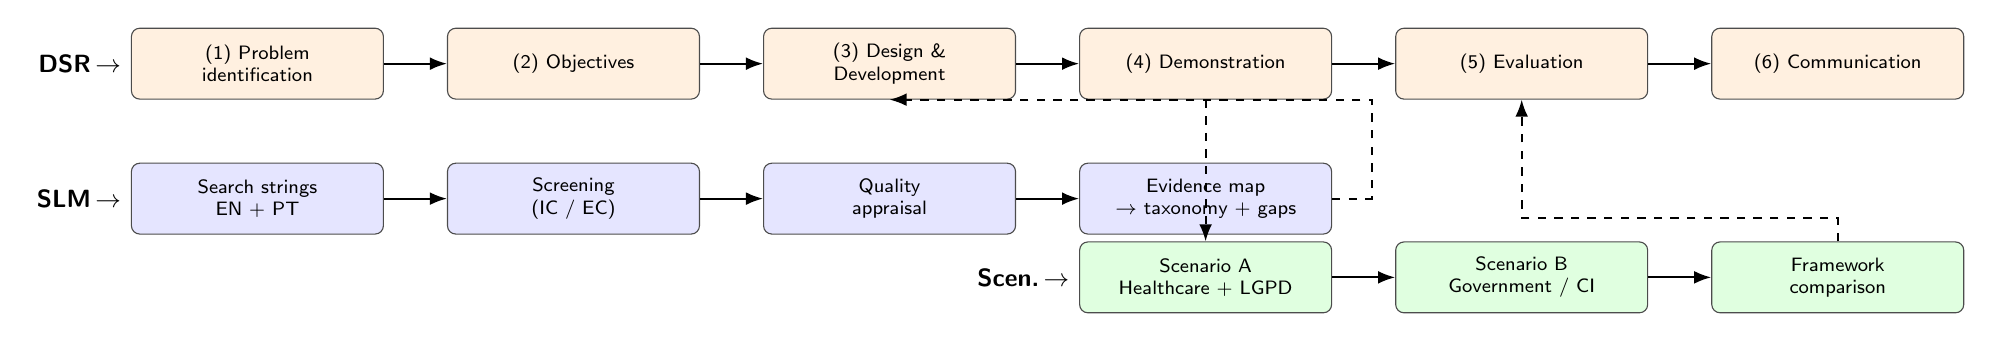
\begin{tikzpicture}[
    node distance=8mm,
    stepbox/.style={rectangle, rounded corners=3pt, draw=black!70,
                 minimum width=3.2cm, minimum height=0.9cm,
                 font=\scriptsize\sffamily, align=center},
    slm/.style={stepbox, fill=blue!10},
    dsr/.style={stepbox, fill=orange!12},
    eval/.style={stepbox, fill=green!12},
    arr/.style={-Latex, line width=0.7pt}
]
  % DSR (top row)
  \node[dsr] (p1) {(1) Problem\\identification};
  \node[dsr, right=of p1] (p2) {(2) Objectives};
  \node[dsr, right=of p2] (p3) {(3) Design \&\\Development};
  \node[dsr, right=of p3] (p4) {(4) Demonstration};
  \node[dsr, right=of p4] (p5) {(5) Evaluation};
  \node[dsr, right=of p5] (p6) {(6) Communication};

  \foreach \a/\b in {p1/p2, p2/p3, p3/p4, p4/p5, p5/p6}{
    \draw[arr] (\a) -- (\b);
  }

  % SLM (below, anchored to p1, p2)
  \node[slm, below=of p1] (s1) {Search strings\\EN + PT};
  \node[slm, right=of s1] (s2) {Screening\\(IC / EC)};
  \node[slm, right=of s2] (s3) {Quality\\appraisal};
  \node[slm, right=of s3] (s4) {Evidence map\\$\rightarrow$ taxonomy + gaps};
  \draw[arr] (s1) -- (s2);
  \draw[arr] (s2) -- (s3);
  \draw[arr] (s3) -- (s4);
  \draw[arr, dashed] (s4.east) -- ++(0.5,0) |- (p3.south);

  % Scenarios (below, anchored to p4, p5)
  \node[eval, below=18mm of p4] (e1) {Scenario A\\Healthcare + LGPD};
  \node[eval, right=of e1]      (e2) {Scenario B\\Government / CI};
  \node[eval, right=of e2]      (e3) {Framework\\comparison};
  \draw[arr] (e1) -- (e2);
  \draw[arr] (e2) -- (e3);
  \draw[arr, dashed] (p4.south) -- ++(0,-0.3) -- (e1.north);
  \draw[arr, dashed] (e3.north) -- ++(0,0.3) -| (p5.south);

  % Labels
  \node[font=\bfseries\small\sffamily, anchor=east] at (p1.west) {DSR\,$\rightarrow$};
  \node[font=\bfseries\small\sffamily, anchor=east] at (s1.west) {SLM\,$\rightarrow$};
  \node[font=\bfseries\small\sffamily, anchor=east] at (e1.west) {Scen.\,$\rightarrow$};
\end{tikzpicture}
% Caption:
% Figure 5. Research method flow. The Design Science Research process (Peffers
% DSRM, top row) is fed by a Systematic Literature Mapping (middle) and
% evaluated by structured scenario analyses (bottom).

\end{document}

%
% Each figure is wrapped in a \begin{figure} block so it can be moved into the
% manuscript at Stage 5 with minor adjustments (positioning/captions).

\documentclass[tikz,border=8pt]{standalone}
\usepackage[utf8]{inputenc}
\usepackage[T1]{fontenc}
\usepackage{tikz}
\usepackage{amsmath,amssymb}
\usetikzlibrary{shapes.geometric,arrows.meta,positioning,fit,backgrounds,
                calc,decorations.pathreplacing,decorations.pathmorphing,
                shadows.blur,patterns}

% ===== Reusable styles =====
\tikzset{
  layer/.style={
    rectangle, rounded corners=4pt, draw=black!70, line width=0.6pt,
    minimum width=11cm, minimum height=1.5cm,
    align=center, font=\small\sffamily, blur shadow={shadow blur steps=3}
  },
  L1/.style={layer, fill=blue!15},
  L2/.style={layer, fill=orange!18},
  L3/.style={layer, fill=green!16},
  L4/.style={layer, fill=red!12},
  flow/.style={-Latex, line width=0.9pt, draw=black!75},
  flowdash/.style={-Latex, line width=0.7pt, draw=black!55, dashed},
  comp/.style={rectangle, rounded corners=3pt, draw=black!65,
               fill=white, minimum width=2.4cm, minimum height=0.7cm,
               font=\footnotesize\sffamily, align=center},
  side/.style={rectangle, rounded corners=2pt, draw=black!60, fill=yellow!18,
               font=\scriptsize\sffamily, align=center,
               minimum width=2.2cm, minimum height=0.55cm},
  label/.style={font=\bfseries\sffamily\small, anchor=west},
  axislbl/.style={font=\footnotesize\itshape, anchor=west}
}

\begin{document}

% =====================================================================
% F1 — SHIELD-AI Four-Layer Architecture
% =====================================================================
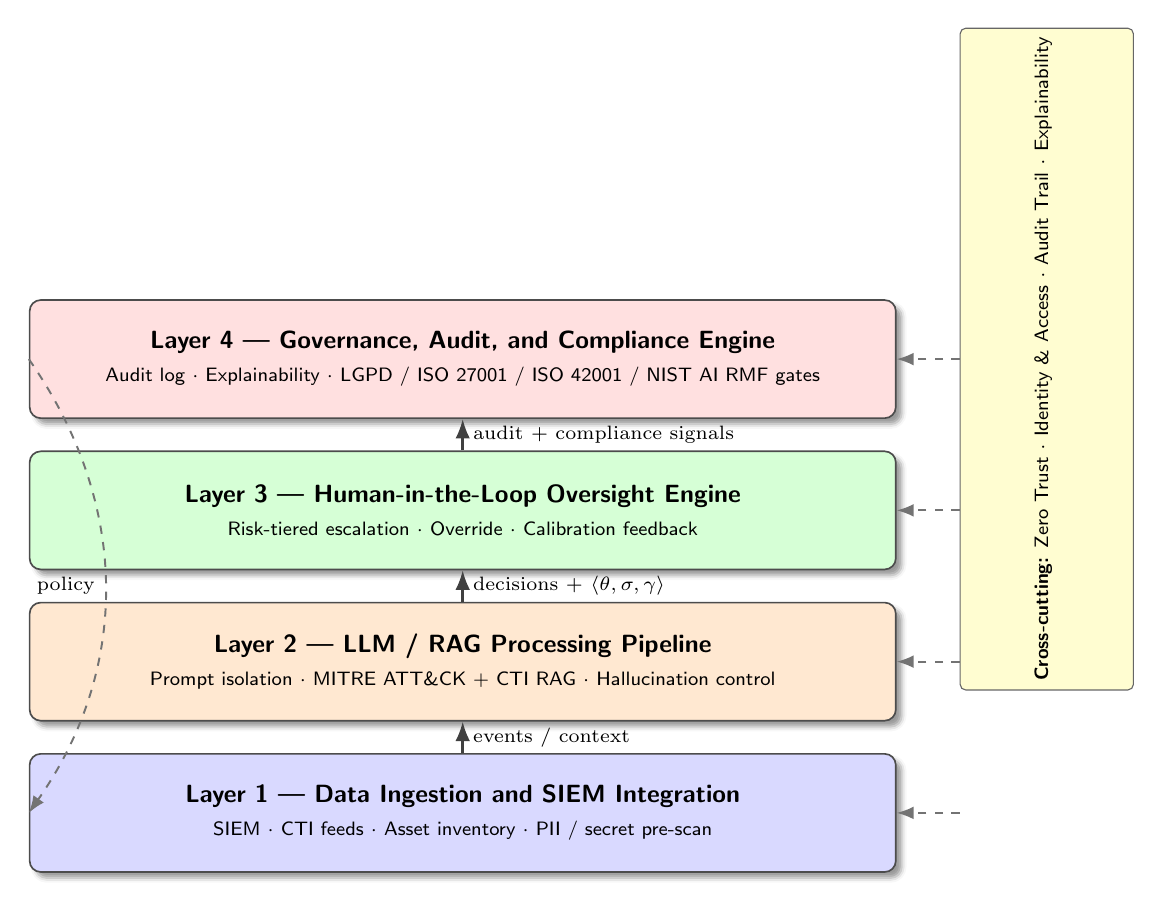
\begin{tikzpicture}[node distance=4mm]
  \node[L4] (L4) {%
    \textbf{Layer 4 — Governance, Audit, and Compliance Engine}\\[1pt]
    \scriptsize Audit log $\cdot$ Explainability $\cdot$ LGPD / ISO 27001 / ISO 42001 / NIST AI RMF gates};
  \node[L3, below=of L4] (L3) {%
    \textbf{Layer 3 — Human-in-the-Loop Oversight Engine}\\[1pt]
    \scriptsize Risk-tiered escalation $\cdot$ Override $\cdot$ Calibration feedback};
  \node[L2, below=of L3] (L2) {%
    \textbf{Layer 2 — LLM / RAG Processing Pipeline}\\[1pt]
    \scriptsize Prompt isolation $\cdot$ MITRE ATT\&CK + CTI RAG $\cdot$ Hallucination control};
  \node[L1, below=of L2] (L1) {%
    \textbf{Layer 1 — Data Ingestion and SIEM Integration}\\[1pt]
    \scriptsize SIEM $\cdot$ CTI feeds $\cdot$ Asset inventory $\cdot$ PII / secret pre-scan};

  % Cross-cutting concerns on the right
  \node[side, right=8mm of L4.east,
        anchor=west, minimum height=8.0cm] (cross) {%
    \rotatebox{90}{\textbf{Cross-cutting:} Zero Trust $\cdot$ Identity \& Access $\cdot$ Audit Trail $\cdot$ Explainability}
  };
  \draw[flowdash] (cross.west|-L4.east) -- (L4.east);
  \draw[flowdash] (cross.west|-L3.east) -- (L3.east);
  \draw[flowdash] (cross.west|-L2.east) -- (L2.east);
  \draw[flowdash] (cross.west|-L1.east) -- (L1.east);

  % Flows between layers
  \draw[flow] (L1.north) -- (L2.south) node[midway, right, font=\scriptsize] {events / context};
  \draw[flow] (L2.north) -- (L3.south) node[midway, right, font=\scriptsize] {decisions + $\langle\theta,\sigma,\gamma\rangle$};
  \draw[flow] (L3.north) -- (L4.south) node[midway, right, font=\scriptsize] {audit + compliance signals};
  \draw[flowdash] (L4.west)+(0,0) to[bend left=35] node[left, font=\scriptsize] {policy} (L1.west);

\end{tikzpicture}
% Caption (for manuscript):
% Figure 1. SHIELD-AI four-layer architecture. Layers are governed top-down by
% standards-aligned policy (L4 → L1) and produce upward flows of events,
% decisions with reliability triples ⟨θ, σ, γ⟩, and audit signals. Cross-cutting
% concerns (Zero Trust, Identity & Access, Audit Trail, Explainability) operate
% across all layers.

% =====================================================================
% F2 — Offensive--Defensive AI Cycle in Cybersecurity
% =====================================================================
\newpage
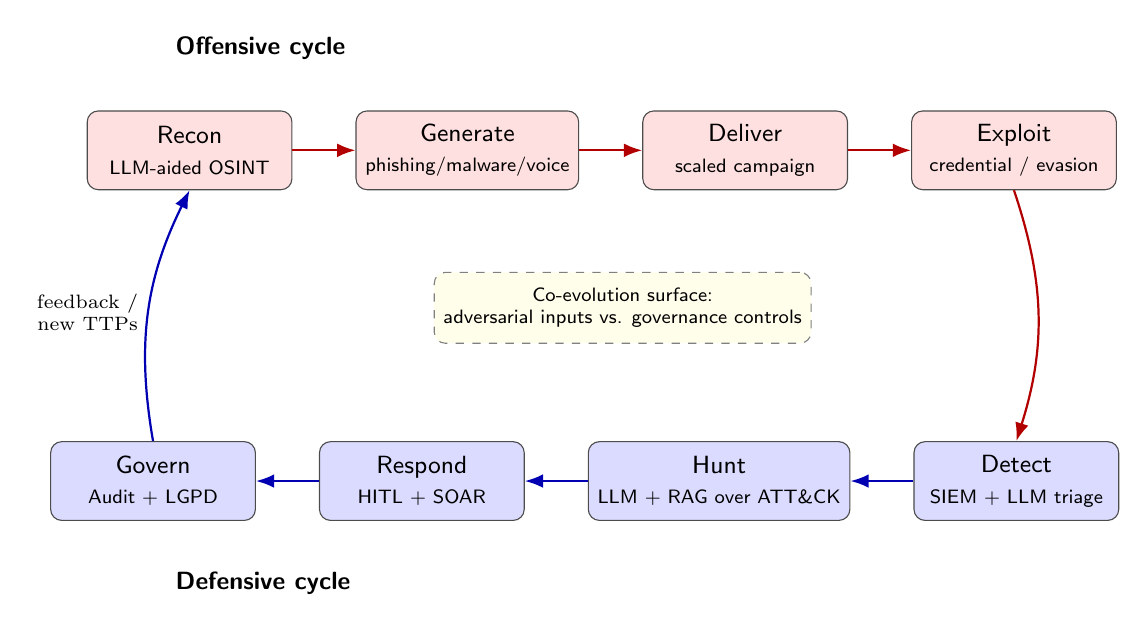
\begin{tikzpicture}[
    node distance=8mm,
    stage/.style={rectangle, rounded corners=4pt, draw=black!70,
                  minimum width=2.6cm, minimum height=1.0cm,
                  align=center, font=\small\sffamily},
    off/.style={stage, fill=red!12},
    def/.style={stage, fill=blue!14},
    cycle/.style={-Latex, line width=0.8pt}
]
  % Offensive stages (top half)
  \node[off] (recon) at (0,3) {Recon\\\scriptsize LLM-aided OSINT};
  \node[off, right=of recon] (gen) {Generate\\\scriptsize phishing/malware/voice};
  \node[off, right=of gen] (deliver) {Deliver\\\scriptsize scaled campaign};
  \node[off, right=of deliver] (exploit) {Exploit\\\scriptsize credential / evasion};

  % Defensive stages (bottom half)
  \node[def] (detect) at (10.5,-1.2) {Detect\\\scriptsize SIEM + LLM triage};
  \node[def, left=of detect] (hunt) {Hunt\\\scriptsize LLM + RAG over ATT\&CK};
  \node[def, left=of hunt] (resp) {Respond\\\scriptsize HITL + SOAR};
  \node[def, left=of resp] (gov) {Govern\\\scriptsize Audit + LGPD};

  % Connecting arrows
  \draw[cycle, draw=red!70!black] (recon) -- (gen);
  \draw[cycle, draw=red!70!black] (gen) -- (deliver);
  \draw[cycle, draw=red!70!black] (deliver) -- (exploit);
  \draw[cycle, draw=red!70!black] (exploit.south) to[bend left=18] (detect.north);

  \draw[cycle, draw=blue!70!black] (detect) -- (hunt);
  \draw[cycle, draw=blue!70!black] (hunt) -- (resp);
  \draw[cycle, draw=blue!70!black] (resp) -- (gov);
  \draw[cycle, draw=blue!70!black] (gov.north) to[bend left=18]
     node[left, font=\scriptsize, align=center] {feedback /\\new TTPs} (recon.south);

  % Central "AI-vs-AI" annotation
  \node[draw=black!50, dashed, rounded corners=4pt,
        fill=yellow!8, font=\scriptsize\sffamily, align=center,
        minimum width=4cm, minimum height=0.9cm] (core) at (5.5,1.0)
        {Co-evolution surface:\\ adversarial inputs vs. governance controls};

  \node[font=\bfseries\sffamily\small, anchor=west] at (-0.3, 4.3) {Offensive cycle};
  \node[font=\bfseries\sffamily\small, anchor=west] at (-0.3, -2.5) {Defensive cycle};

\end{tikzpicture}
% Caption:
% Figure 2. Offensive--defensive AI co-evolution. Generative AI accelerates
% adversary operations (top); defensive AI must accelerate detection, hunting,
% response, and governance (bottom). The two cycles share a co-evolution
% surface, including prompt-injection and tool-poisoning vectors against the
% defensive AI itself.

% =====================================================================
% F3 — SOC Pipeline (Data Flow Detail)
% =====================================================================
\newpage
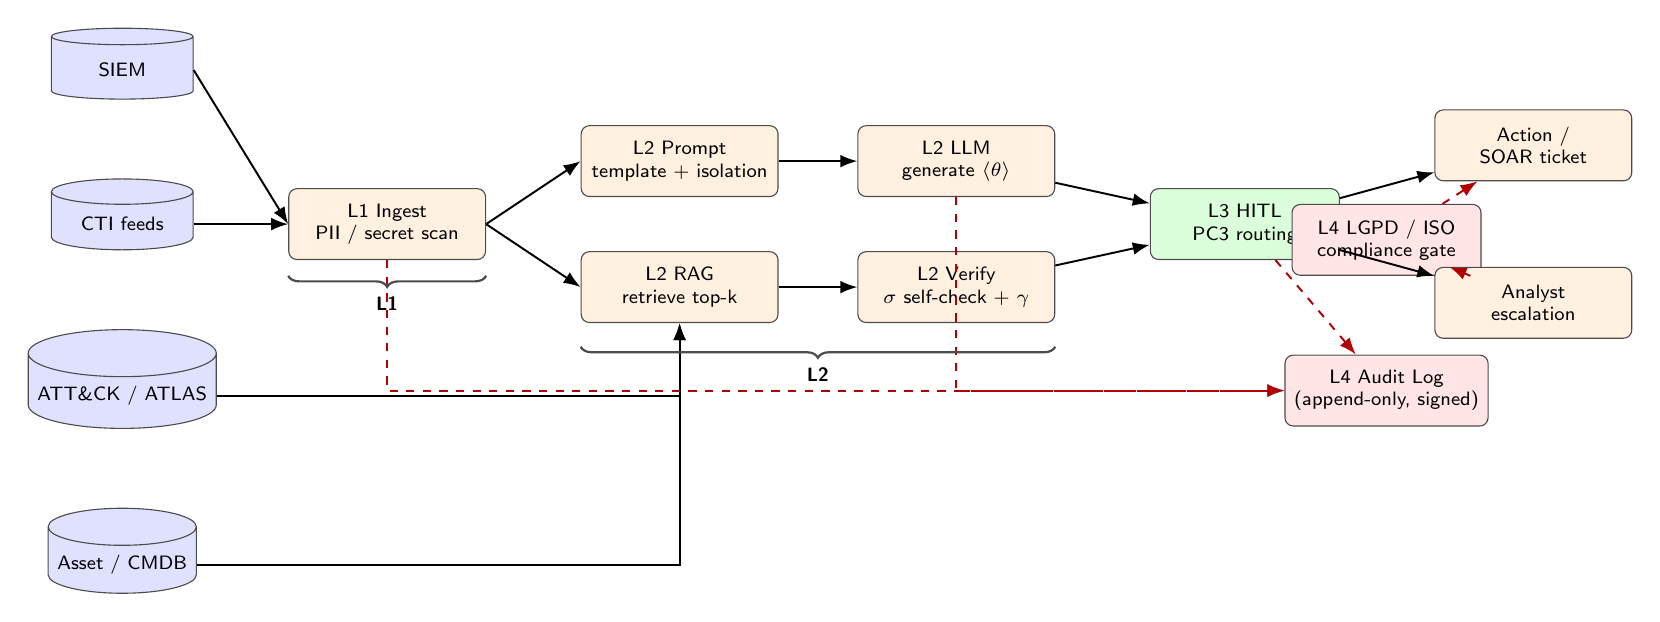
\begin{tikzpicture}[node distance=10mm,
    src/.style={cylinder, shape border rotate=90, aspect=0.25,
                draw=black!70, fill=blue!12, minimum height=0.9cm,
                minimum width=1.8cm, font=\scriptsize\sffamily, align=center},
    blk/.style={rectangle, rounded corners=3pt, draw=black!70,
                fill=orange!12, minimum width=2.5cm, minimum height=0.9cm,
                font=\scriptsize\sffamily, align=center},
    eng/.style={rectangle, rounded corners=3pt, draw=black!70,
                fill=green!14, minimum width=2.4cm, minimum height=0.9cm,
                font=\scriptsize\sffamily, align=center},
    gov/.style={rectangle, rounded corners=3pt, draw=black!70,
                fill=red!10, minimum width=2.4cm, minimum height=0.9cm,
                font=\scriptsize\sffamily, align=center},
    arr/.style={-Latex, line width=0.7pt}
]
  % Sources (left column)
  \node[src] (siem) {SIEM};
  \node[src, below=of siem] (cti)  {CTI feeds};
  \node[src, below=of cti]  (attck){ATT\&CK / ATLAS};
  \node[src, below=of attck] (cmdb){Asset / CMDB};

  % L1
  \node[blk, right=12mm of cti] (ingest) {L1 Ingest\\PII / secret scan};

  % L2 LLM/RAG pipeline
  \node[blk, right=12mm of ingest, yshift=8mm]  (prompt) {L2 Prompt\\template + isolation};
  \node[blk, right=12mm of ingest, yshift=-8mm] (rag)    {L2 RAG\\retrieve top-k};
  \node[blk, right=of prompt] (llm) {L2 LLM\\generate $\langle\theta\rangle$};
  \node[blk, right=of rag]    (check){L2 Verify\\$\sigma$ self-check + $\gamma$};

  % L3 HITL
  \node[eng, right=12mm of llm, yshift=-8mm] (hitl) {L3 HITL\\PC3 routing};

  % L4 Governance
  \node[gov, below=12mm of hitl, xshift=18mm] (audit) {L4 Audit Log\\(append-only, signed)};
  \node[gov, above=of audit] (compl) {L4 LGPD / ISO\\ compliance gate};

  % Final outputs
  \node[blk, right=12mm of hitl, yshift=10mm] (action) {Action /\\SOAR ticket};
  \node[blk, right=12mm of hitl, yshift=-10mm](escal)  {Analyst\\escalation};

  % Arrows
  \draw[arr] (siem.east)  -- (ingest.west);
  \draw[arr] (cti.east)   -- (ingest.west);
  \draw[arr] (attck.east) -| (rag.south);
  \draw[arr] (cmdb.east)  -| (rag.south);
  \draw[arr] (ingest.east) -- (prompt.west);
  \draw[arr] (ingest.east) -- (rag.west);
  \draw[arr] (prompt) -- (llm);
  \draw[arr] (rag) -- (check);
  \draw[arr] (llm) -- (hitl);
  \draw[arr] (check) -- (hitl);
  \draw[arr] (hitl) -- (action);
  \draw[arr] (hitl) -- (escal);

  % L4 governance arrows (dashed, two-way)
  \draw[arr, dashed, draw=red!70!black] (hitl) -- (audit);
  \draw[arr, dashed, draw=red!70!black] (llm) |- (audit);
  \draw[arr, dashed, draw=red!70!black] (ingest) |- (audit);
  \draw[arr, dashed, draw=red!70!black] (compl) -- (action);
  \draw[arr, dashed, draw=red!70!black] (compl) -- (escal);

  % Layer brackets
  \draw[decorate, decoration={brace, amplitude=4pt, mirror},
        line width=0.8pt, draw=black!70]
       ($(ingest.south west)+(0,-0.2)$) -- ($(ingest.south east)+(0,-0.2)$)
       node[midway, below=4pt, font=\bfseries\scriptsize\sffamily] {L1};
  \draw[decorate, decoration={brace, amplitude=4pt, mirror},
        line width=0.8pt, draw=black!70]
       ($(rag.south west)+(0,-0.3)$) -- ($(check.south east)+(0,-0.3)$)
       node[midway, below=4pt, font=\bfseries\scriptsize\sffamily] {L2};
\end{tikzpicture}
% Caption:
% Figure 3. SHIELD-AI SOC pipeline detail. L1 ingests events from SIEM, CTI,
% and asset inventory with PII pre-scanning. L2 isolates prompt and data, runs
% RAG over MITRE ATT&CK/ATLAS, and computes the reliability triple ⟨θ, σ, γ⟩.
% L3 routes outputs through PC3 (auto / HITL / reject). L4 records every step
% in an append-only audit log and gates outgoing actions against LGPD and ISO
% requirements.

% =====================================================================
% F4 — Governance and Audit Model
% =====================================================================
\newpage
\begin{tikzpicture}[
    node distance=7mm,
    obj/.style={rectangle, rounded corners=3pt, draw=black!70,
                minimum width=3.2cm, minimum height=0.9cm,
                font=\scriptsize\sffamily, align=center},
    invar/.style={obj, fill=red!12},
    ctrl/.style={obj, fill=orange!14},
    std/.style={obj, fill=blue!12},
    arr/.style={-Latex, line width=0.7pt}
]
  % Center: audit invariant
  \node[invar, minimum width=5.6cm, minimum height=1.2cm] (A)
       {\textbf{Audit Invariant 𝓐} \\
        $\langle$input, prompt, retrieved, output, $\theta,\sigma,\gamma$, route, analyst, ts$\rangle$};

  % Controls feeding into 𝓐
  \node[ctrl, above left=of A] (c1) {Input sanitization};
  \node[ctrl, above=of A]      (c2) {Self-check + RAG verification};
  \node[ctrl, above right=of A](c3) {HITL routing};
  \node[ctrl, below left=of A] (c4) {Tool allowlist};
  \node[ctrl, below=of A]      (c5) {LGPD / PII gate};
  \node[ctrl, below right=of A](c6) {Identity / Zero-Trust};

  \foreach \c in {c1,c2,c3,c4,c5,c6}{
    \draw[arr] (\c) -- (A);
  }

  % Standards arrayed on right (𝓜 mapping) — extra horizontal space avoids label overlap
  \node[std, right=42mm of A.east, yshift=22mm] (s1) {MITRE ATT\&CK / ATLAS};
  \node[std, right=42mm of A.east, yshift= 8mm] (s2) {NIST CSF 2.0 / AI RMF};
  \node[std, right=42mm of A.east, yshift=-6mm] (s3) {OWASP LLM \& Agentic};
  \node[std, right=42mm of A.east, yshift=-20mm](s4) {ISO 27001 / 42001 / LGPD};

  % Mapping 𝓜 arrows from controls to standards — route around control labels
  \draw[arr, draw=blue!60!black, dashed] (c3.east) -- ++(0.6,0) |- (s1.west);
  \draw[arr, draw=blue!60!black, dashed] (c2.north east) -- ++(0.4,0) |- (s1.west);
  \draw[arr, draw=blue!60!black, dashed] (c1.east) -- ++(0.6,0) |- (s3.west);
  \draw[arr, draw=blue!60!black, dashed] (c5.east) -- ++(0.6,0) |- (s4.west);
  \draw[arr, draw=blue!60!black, dashed] (c6.east) -- ++(0.6,0) |- (s2.west);

  % Property output
  \node[obj, fill=green!14, left=18mm of A.west] (P) {Properties 𝓟\\(P1--P7)};
  \draw[arr, draw=green!60!black] (A) -- (P);

  \node[font=\itshape\scriptsize\sffamily, anchor=north, text width=4cm]
    at ($(P.south)+(0,-1mm)$)
    {Audit-complete $\cdot$ CGS-monotone $\cdot$ Compliance-preserving $\cdot$ Policy-derivable HITL};

\end{tikzpicture}
% Caption:
% Figure 4. Governance and audit model. Controls (orange) emit audit tuples
% into the invariant 𝓐 (red center). The mapping 𝓜 (dashed blue) routes each
% control to its corresponding external standards. Properties 𝓟 (green, left)
% are guaranteed by construction (see Lemmas 1--2 and Theorems 1--3).

% =====================================================================
% F5 — Research Method Flow (DSR + SLM + Scenario Evaluation)
% =====================================================================
\newpage
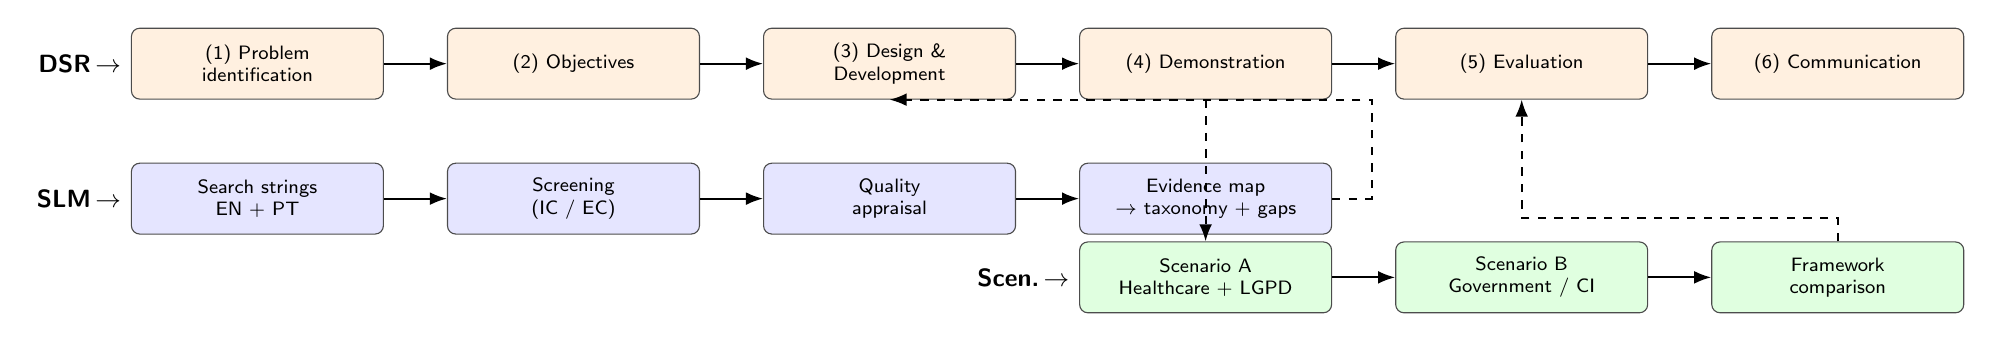
\begin{tikzpicture}[
    node distance=8mm,
    stepbox/.style={rectangle, rounded corners=3pt, draw=black!70,
                 minimum width=3.2cm, minimum height=0.9cm,
                 font=\scriptsize\sffamily, align=center},
    slm/.style={stepbox, fill=blue!10},
    dsr/.style={stepbox, fill=orange!12},
    eval/.style={stepbox, fill=green!12},
    arr/.style={-Latex, line width=0.7pt}
]
  % DSR (top row)
  \node[dsr] (p1) {(1) Problem\\identification};
  \node[dsr, right=of p1] (p2) {(2) Objectives};
  \node[dsr, right=of p2] (p3) {(3) Design \&\\Development};
  \node[dsr, right=of p3] (p4) {(4) Demonstration};
  \node[dsr, right=of p4] (p5) {(5) Evaluation};
  \node[dsr, right=of p5] (p6) {(6) Communication};

  \foreach \a/\b in {p1/p2, p2/p3, p3/p4, p4/p5, p5/p6}{
    \draw[arr] (\a) -- (\b);
  }

  % SLM (below, anchored to p1, p2)
  \node[slm, below=of p1] (s1) {Search strings\\EN + PT};
  \node[slm, right=of s1] (s2) {Screening\\(IC / EC)};
  \node[slm, right=of s2] (s3) {Quality\\appraisal};
  \node[slm, right=of s3] (s4) {Evidence map\\$\rightarrow$ taxonomy + gaps};
  \draw[arr] (s1) -- (s2);
  \draw[arr] (s2) -- (s3);
  \draw[arr] (s3) -- (s4);
  \draw[arr, dashed] (s4.east) -- ++(0.5,0) |- (p3.south);

  % Scenarios (below, anchored to p4, p5)
  \node[eval, below=18mm of p4] (e1) {Scenario A\\Healthcare + LGPD};
  \node[eval, right=of e1]      (e2) {Scenario B\\Government / CI};
  \node[eval, right=of e2]      (e3) {Framework\\comparison};
  \draw[arr] (e1) -- (e2);
  \draw[arr] (e2) -- (e3);
  \draw[arr, dashed] (p4.south) -- ++(0,-0.3) -- (e1.north);
  \draw[arr, dashed] (e3.north) -- ++(0,0.3) -| (p5.south);

  % Labels
  \node[font=\bfseries\small\sffamily, anchor=east] at (p1.west) {DSR\,$\rightarrow$};
  \node[font=\bfseries\small\sffamily, anchor=east] at (s1.west) {SLM\,$\rightarrow$};
  \node[font=\bfseries\small\sffamily, anchor=east] at (e1.west) {Scen.\,$\rightarrow$};
\end{tikzpicture}
% Caption:
% Figure 5. Research method flow. The Design Science Research process (Peffers
% DSRM, top row) is fed by a Systematic Literature Mapping (middle) and
% evaluated by structured scenario analyses (bottom).

\end{document}

%
% Each figure is wrapped in a \begin{figure} block so it can be moved into the
% manuscript at Stage 5 with minor adjustments (positioning/captions).

\documentclass[tikz,border=8pt]{standalone}
\usepackage[utf8]{inputenc}
\usepackage[T1]{fontenc}
\usepackage{tikz}
\usepackage{amsmath,amssymb}
\usetikzlibrary{shapes.geometric,arrows.meta,positioning,fit,backgrounds,
                calc,decorations.pathreplacing,decorations.pathmorphing,
                shadows.blur,patterns}

% ===== Reusable styles =====
\tikzset{
  layer/.style={
    rectangle, rounded corners=4pt, draw=black!70, line width=0.6pt,
    minimum width=11cm, minimum height=1.5cm,
    align=center, font=\small\sffamily, blur shadow={shadow blur steps=3}
  },
  L1/.style={layer, fill=blue!15},
  L2/.style={layer, fill=orange!18},
  L3/.style={layer, fill=green!16},
  L4/.style={layer, fill=red!12},
  flow/.style={-Latex, line width=0.9pt, draw=black!75},
  flowdash/.style={-Latex, line width=0.7pt, draw=black!55, dashed},
  comp/.style={rectangle, rounded corners=3pt, draw=black!65,
               fill=white, minimum width=2.4cm, minimum height=0.7cm,
               font=\footnotesize\sffamily, align=center},
  side/.style={rectangle, rounded corners=2pt, draw=black!60, fill=yellow!18,
               font=\scriptsize\sffamily, align=center,
               minimum width=2.2cm, minimum height=0.55cm},
  label/.style={font=\bfseries\sffamily\small, anchor=west},
  axislbl/.style={font=\footnotesize\itshape, anchor=west}
}

\begin{document}

% =====================================================================
% F1 — SHIELD-AI Four-Layer Architecture
% =====================================================================
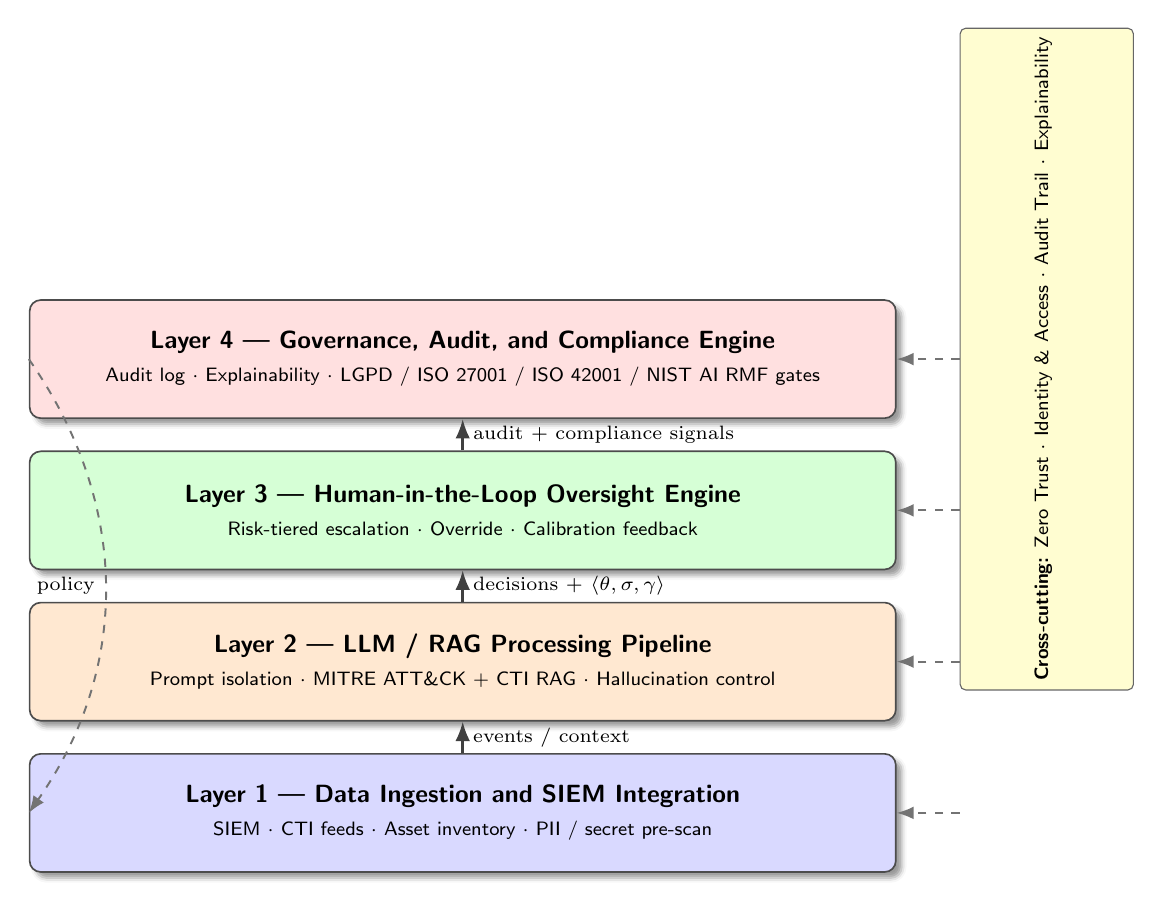
\begin{tikzpicture}[node distance=4mm]
  \node[L4] (L4) {%
    \textbf{Layer 4 — Governance, Audit, and Compliance Engine}\\[1pt]
    \scriptsize Audit log $\cdot$ Explainability $\cdot$ LGPD / ISO 27001 / ISO 42001 / NIST AI RMF gates};
  \node[L3, below=of L4] (L3) {%
    \textbf{Layer 3 — Human-in-the-Loop Oversight Engine}\\[1pt]
    \scriptsize Risk-tiered escalation $\cdot$ Override $\cdot$ Calibration feedback};
  \node[L2, below=of L3] (L2) {%
    \textbf{Layer 2 — LLM / RAG Processing Pipeline}\\[1pt]
    \scriptsize Prompt isolation $\cdot$ MITRE ATT\&CK + CTI RAG $\cdot$ Hallucination control};
  \node[L1, below=of L2] (L1) {%
    \textbf{Layer 1 — Data Ingestion and SIEM Integration}\\[1pt]
    \scriptsize SIEM $\cdot$ CTI feeds $\cdot$ Asset inventory $\cdot$ PII / secret pre-scan};

  % Cross-cutting concerns on the right
  \node[side, right=8mm of L4.east,
        anchor=west, minimum height=8.0cm] (cross) {%
    \rotatebox{90}{\textbf{Cross-cutting:} Zero Trust $\cdot$ Identity \& Access $\cdot$ Audit Trail $\cdot$ Explainability}
  };
  \draw[flowdash] (cross.west|-L4.east) -- (L4.east);
  \draw[flowdash] (cross.west|-L3.east) -- (L3.east);
  \draw[flowdash] (cross.west|-L2.east) -- (L2.east);
  \draw[flowdash] (cross.west|-L1.east) -- (L1.east);

  % Flows between layers
  \draw[flow] (L1.north) -- (L2.south) node[midway, right, font=\scriptsize] {events / context};
  \draw[flow] (L2.north) -- (L3.south) node[midway, right, font=\scriptsize] {decisions + $\langle\theta,\sigma,\gamma\rangle$};
  \draw[flow] (L3.north) -- (L4.south) node[midway, right, font=\scriptsize] {audit + compliance signals};
  \draw[flowdash] (L4.west)+(0,0) to[bend left=35] node[left, font=\scriptsize] {policy} (L1.west);

\end{tikzpicture}
% Caption (for manuscript):
% Figure 1. SHIELD-AI four-layer architecture. Layers are governed top-down by
% standards-aligned policy (L4 → L1) and produce upward flows of events,
% decisions with reliability triples ⟨θ, σ, γ⟩, and audit signals. Cross-cutting
% concerns (Zero Trust, Identity & Access, Audit Trail, Explainability) operate
% across all layers.

% =====================================================================
% F2 — Offensive--Defensive AI Cycle in Cybersecurity
% =====================================================================
\newpage
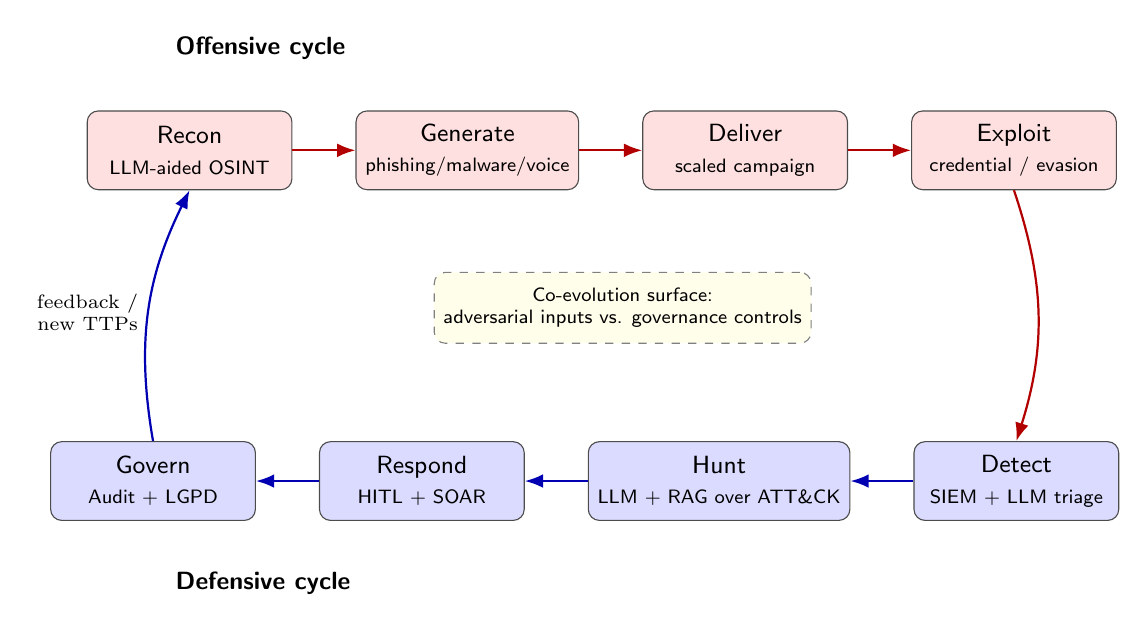
\begin{tikzpicture}[
    node distance=8mm,
    stage/.style={rectangle, rounded corners=4pt, draw=black!70,
                  minimum width=2.6cm, minimum height=1.0cm,
                  align=center, font=\small\sffamily},
    off/.style={stage, fill=red!12},
    def/.style={stage, fill=blue!14},
    cycle/.style={-Latex, line width=0.8pt}
]
  % Offensive stages (top half)
  \node[off] (recon) at (0,3) {Recon\\\scriptsize LLM-aided OSINT};
  \node[off, right=of recon] (gen) {Generate\\\scriptsize phishing/malware/voice};
  \node[off, right=of gen] (deliver) {Deliver\\\scriptsize scaled campaign};
  \node[off, right=of deliver] (exploit) {Exploit\\\scriptsize credential / evasion};

  % Defensive stages (bottom half)
  \node[def] (detect) at (10.5,-1.2) {Detect\\\scriptsize SIEM + LLM triage};
  \node[def, left=of detect] (hunt) {Hunt\\\scriptsize LLM + RAG over ATT\&CK};
  \node[def, left=of hunt] (resp) {Respond\\\scriptsize HITL + SOAR};
  \node[def, left=of resp] (gov) {Govern\\\scriptsize Audit + LGPD};

  % Connecting arrows
  \draw[cycle, draw=red!70!black] (recon) -- (gen);
  \draw[cycle, draw=red!70!black] (gen) -- (deliver);
  \draw[cycle, draw=red!70!black] (deliver) -- (exploit);
  \draw[cycle, draw=red!70!black] (exploit.south) to[bend left=18] (detect.north);

  \draw[cycle, draw=blue!70!black] (detect) -- (hunt);
  \draw[cycle, draw=blue!70!black] (hunt) -- (resp);
  \draw[cycle, draw=blue!70!black] (resp) -- (gov);
  \draw[cycle, draw=blue!70!black] (gov.north) to[bend left=18]
     node[left, font=\scriptsize, align=center] {feedback /\\new TTPs} (recon.south);

  % Central "AI-vs-AI" annotation
  \node[draw=black!50, dashed, rounded corners=4pt,
        fill=yellow!8, font=\scriptsize\sffamily, align=center,
        minimum width=4cm, minimum height=0.9cm] (core) at (5.5,1.0)
        {Co-evolution surface:\\ adversarial inputs vs. governance controls};

  \node[font=\bfseries\sffamily\small, anchor=west] at (-0.3, 4.3) {Offensive cycle};
  \node[font=\bfseries\sffamily\small, anchor=west] at (-0.3, -2.5) {Defensive cycle};

\end{tikzpicture}
% Caption:
% Figure 2. Offensive--defensive AI co-evolution. Generative AI accelerates
% adversary operations (top); defensive AI must accelerate detection, hunting,
% response, and governance (bottom). The two cycles share a co-evolution
% surface, including prompt-injection and tool-poisoning vectors against the
% defensive AI itself.

% =====================================================================
% F3 — SOC Pipeline (Data Flow Detail)
% =====================================================================
\newpage
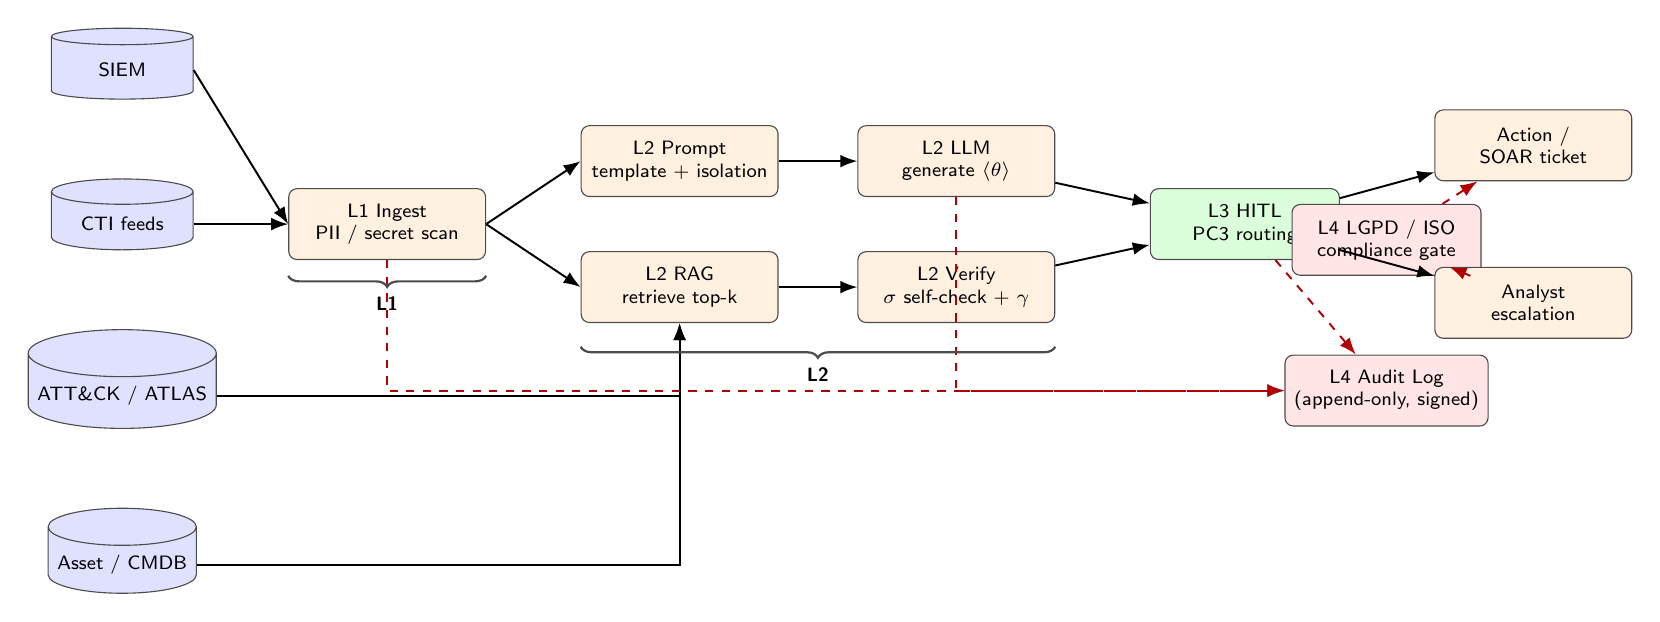
\begin{tikzpicture}[node distance=10mm,
    src/.style={cylinder, shape border rotate=90, aspect=0.25,
                draw=black!70, fill=blue!12, minimum height=0.9cm,
                minimum width=1.8cm, font=\scriptsize\sffamily, align=center},
    blk/.style={rectangle, rounded corners=3pt, draw=black!70,
                fill=orange!12, minimum width=2.5cm, minimum height=0.9cm,
                font=\scriptsize\sffamily, align=center},
    eng/.style={rectangle, rounded corners=3pt, draw=black!70,
                fill=green!14, minimum width=2.4cm, minimum height=0.9cm,
                font=\scriptsize\sffamily, align=center},
    gov/.style={rectangle, rounded corners=3pt, draw=black!70,
                fill=red!10, minimum width=2.4cm, minimum height=0.9cm,
                font=\scriptsize\sffamily, align=center},
    arr/.style={-Latex, line width=0.7pt}
]
  % Sources (left column)
  \node[src] (siem) {SIEM};
  \node[src, below=of siem] (cti)  {CTI feeds};
  \node[src, below=of cti]  (attck){ATT\&CK / ATLAS};
  \node[src, below=of attck] (cmdb){Asset / CMDB};

  % L1
  \node[blk, right=12mm of cti] (ingest) {L1 Ingest\\PII / secret scan};

  % L2 LLM/RAG pipeline
  \node[blk, right=12mm of ingest, yshift=8mm]  (prompt) {L2 Prompt\\template + isolation};
  \node[blk, right=12mm of ingest, yshift=-8mm] (rag)    {L2 RAG\\retrieve top-k};
  \node[blk, right=of prompt] (llm) {L2 LLM\\generate $\langle\theta\rangle$};
  \node[blk, right=of rag]    (check){L2 Verify\\$\sigma$ self-check + $\gamma$};

  % L3 HITL
  \node[eng, right=12mm of llm, yshift=-8mm] (hitl) {L3 HITL\\PC3 routing};

  % L4 Governance
  \node[gov, below=12mm of hitl, xshift=18mm] (audit) {L4 Audit Log\\(append-only, signed)};
  \node[gov, above=of audit] (compl) {L4 LGPD / ISO\\ compliance gate};

  % Final outputs
  \node[blk, right=12mm of hitl, yshift=10mm] (action) {Action /\\SOAR ticket};
  \node[blk, right=12mm of hitl, yshift=-10mm](escal)  {Analyst\\escalation};

  % Arrows
  \draw[arr] (siem.east)  -- (ingest.west);
  \draw[arr] (cti.east)   -- (ingest.west);
  \draw[arr] (attck.east) -| (rag.south);
  \draw[arr] (cmdb.east)  -| (rag.south);
  \draw[arr] (ingest.east) -- (prompt.west);
  \draw[arr] (ingest.east) -- (rag.west);
  \draw[arr] (prompt) -- (llm);
  \draw[arr] (rag) -- (check);
  \draw[arr] (llm) -- (hitl);
  \draw[arr] (check) -- (hitl);
  \draw[arr] (hitl) -- (action);
  \draw[arr] (hitl) -- (escal);

  % L4 governance arrows (dashed, two-way)
  \draw[arr, dashed, draw=red!70!black] (hitl) -- (audit);
  \draw[arr, dashed, draw=red!70!black] (llm) |- (audit);
  \draw[arr, dashed, draw=red!70!black] (ingest) |- (audit);
  \draw[arr, dashed, draw=red!70!black] (compl) -- (action);
  \draw[arr, dashed, draw=red!70!black] (compl) -- (escal);

  % Layer brackets
  \draw[decorate, decoration={brace, amplitude=4pt, mirror},
        line width=0.8pt, draw=black!70]
       ($(ingest.south west)+(0,-0.2)$) -- ($(ingest.south east)+(0,-0.2)$)
       node[midway, below=4pt, font=\bfseries\scriptsize\sffamily] {L1};
  \draw[decorate, decoration={brace, amplitude=4pt, mirror},
        line width=0.8pt, draw=black!70]
       ($(rag.south west)+(0,-0.3)$) -- ($(check.south east)+(0,-0.3)$)
       node[midway, below=4pt, font=\bfseries\scriptsize\sffamily] {L2};
\end{tikzpicture}
% Caption:
% Figure 3. SHIELD-AI SOC pipeline detail. L1 ingests events from SIEM, CTI,
% and asset inventory with PII pre-scanning. L2 isolates prompt and data, runs
% RAG over MITRE ATT&CK/ATLAS, and computes the reliability triple ⟨θ, σ, γ⟩.
% L3 routes outputs through PC3 (auto / HITL / reject). L4 records every step
% in an append-only audit log and gates outgoing actions against LGPD and ISO
% requirements.

% =====================================================================
% F4 — Governance and Audit Model
% =====================================================================
\newpage
\begin{tikzpicture}[
    node distance=7mm,
    obj/.style={rectangle, rounded corners=3pt, draw=black!70,
                minimum width=3.2cm, minimum height=0.9cm,
                font=\scriptsize\sffamily, align=center},
    invar/.style={obj, fill=red!12},
    ctrl/.style={obj, fill=orange!14},
    std/.style={obj, fill=blue!12},
    arr/.style={-Latex, line width=0.7pt}
]
  % Center: audit invariant
  \node[invar, minimum width=5.6cm, minimum height=1.2cm] (A)
       {\textbf{Audit Invariant 𝓐} \\
        $\langle$input, prompt, retrieved, output, $\theta,\sigma,\gamma$, route, analyst, ts$\rangle$};

  % Controls feeding into 𝓐
  \node[ctrl, above left=of A] (c1) {Input sanitization};
  \node[ctrl, above=of A]      (c2) {Self-check + RAG verification};
  \node[ctrl, above right=of A](c3) {HITL routing};
  \node[ctrl, below left=of A] (c4) {Tool allowlist};
  \node[ctrl, below=of A]      (c5) {LGPD / PII gate};
  \node[ctrl, below right=of A](c6) {Identity / Zero-Trust};

  \foreach \c in {c1,c2,c3,c4,c5,c6}{
    \draw[arr] (\c) -- (A);
  }

  % Standards arrayed on right (𝓜 mapping) — extra horizontal space avoids label overlap
  \node[std, right=42mm of A.east, yshift=22mm] (s1) {MITRE ATT\&CK / ATLAS};
  \node[std, right=42mm of A.east, yshift= 8mm] (s2) {NIST CSF 2.0 / AI RMF};
  \node[std, right=42mm of A.east, yshift=-6mm] (s3) {OWASP LLM \& Agentic};
  \node[std, right=42mm of A.east, yshift=-20mm](s4) {ISO 27001 / 42001 / LGPD};

  % Mapping 𝓜 arrows from controls to standards — route around control labels
  \draw[arr, draw=blue!60!black, dashed] (c3.east) -- ++(0.6,0) |- (s1.west);
  \draw[arr, draw=blue!60!black, dashed] (c2.north east) -- ++(0.4,0) |- (s1.west);
  \draw[arr, draw=blue!60!black, dashed] (c1.east) -- ++(0.6,0) |- (s3.west);
  \draw[arr, draw=blue!60!black, dashed] (c5.east) -- ++(0.6,0) |- (s4.west);
  \draw[arr, draw=blue!60!black, dashed] (c6.east) -- ++(0.6,0) |- (s2.west);

  % Property output
  \node[obj, fill=green!14, left=18mm of A.west] (P) {Properties 𝓟\\(P1--P7)};
  \draw[arr, draw=green!60!black] (A) -- (P);

  \node[font=\itshape\scriptsize\sffamily, anchor=north, text width=4cm]
    at ($(P.south)+(0,-1mm)$)
    {Audit-complete $\cdot$ CGS-monotone $\cdot$ Compliance-preserving $\cdot$ Policy-derivable HITL};

\end{tikzpicture}
% Caption:
% Figure 4. Governance and audit model. Controls (orange) emit audit tuples
% into the invariant 𝓐 (red center). The mapping 𝓜 (dashed blue) routes each
% control to its corresponding external standards. Properties 𝓟 (green, left)
% are guaranteed by construction (see Lemmas 1--2 and Theorems 1--3).

% =====================================================================
% F5 — Research Method Flow (DSR + SLM + Scenario Evaluation)
% =====================================================================
\newpage
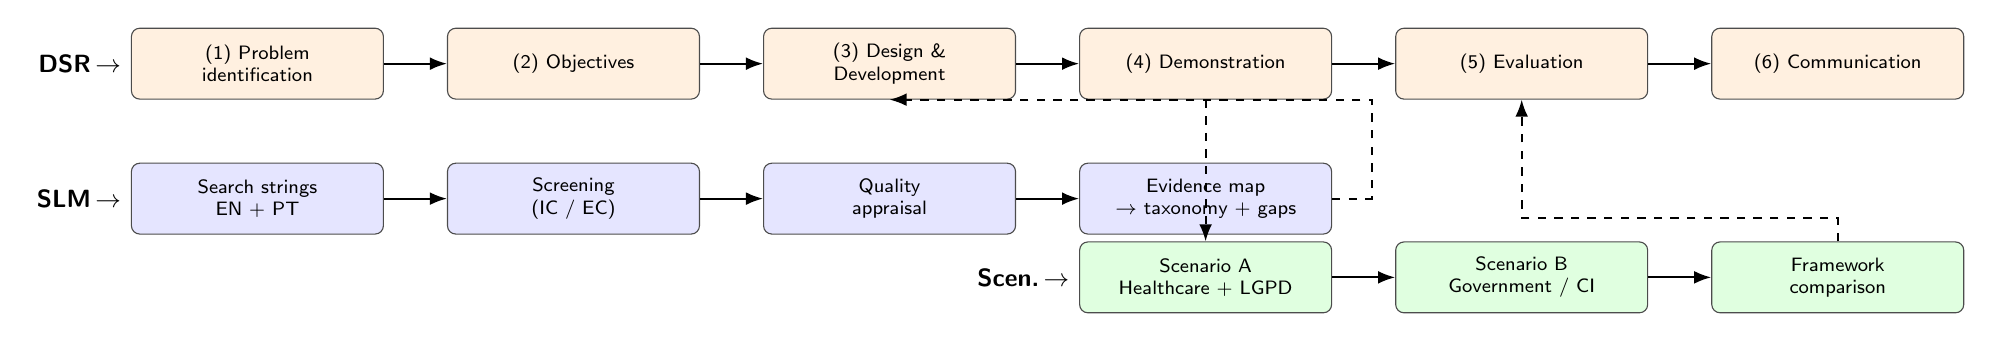
\begin{tikzpicture}[
    node distance=8mm,
    stepbox/.style={rectangle, rounded corners=3pt, draw=black!70,
                 minimum width=3.2cm, minimum height=0.9cm,
                 font=\scriptsize\sffamily, align=center},
    slm/.style={stepbox, fill=blue!10},
    dsr/.style={stepbox, fill=orange!12},
    eval/.style={stepbox, fill=green!12},
    arr/.style={-Latex, line width=0.7pt}
]
  % DSR (top row)
  \node[dsr] (p1) {(1) Problem\\identification};
  \node[dsr, right=of p1] (p2) {(2) Objectives};
  \node[dsr, right=of p2] (p3) {(3) Design \&\\Development};
  \node[dsr, right=of p3] (p4) {(4) Demonstration};
  \node[dsr, right=of p4] (p5) {(5) Evaluation};
  \node[dsr, right=of p5] (p6) {(6) Communication};

  \foreach \a/\b in {p1/p2, p2/p3, p3/p4, p4/p5, p5/p6}{
    \draw[arr] (\a) -- (\b);
  }

  % SLM (below, anchored to p1, p2)
  \node[slm, below=of p1] (s1) {Search strings\\EN + PT};
  \node[slm, right=of s1] (s2) {Screening\\(IC / EC)};
  \node[slm, right=of s2] (s3) {Quality\\appraisal};
  \node[slm, right=of s3] (s4) {Evidence map\\$\rightarrow$ taxonomy + gaps};
  \draw[arr] (s1) -- (s2);
  \draw[arr] (s2) -- (s3);
  \draw[arr] (s3) -- (s4);
  \draw[arr, dashed] (s4.east) -- ++(0.5,0) |- (p3.south);

  % Scenarios (below, anchored to p4, p5)
  \node[eval, below=18mm of p4] (e1) {Scenario A\\Healthcare + LGPD};
  \node[eval, right=of e1]      (e2) {Scenario B\\Government / CI};
  \node[eval, right=of e2]      (e3) {Framework\\comparison};
  \draw[arr] (e1) -- (e2);
  \draw[arr] (e2) -- (e3);
  \draw[arr, dashed] (p4.south) -- ++(0,-0.3) -- (e1.north);
  \draw[arr, dashed] (e3.north) -- ++(0,0.3) -| (p5.south);

  % Labels
  \node[font=\bfseries\small\sffamily, anchor=east] at (p1.west) {DSR\,$\rightarrow$};
  \node[font=\bfseries\small\sffamily, anchor=east] at (s1.west) {SLM\,$\rightarrow$};
  \node[font=\bfseries\small\sffamily, anchor=east] at (e1.west) {Scen.\,$\rightarrow$};
\end{tikzpicture}
% Caption:
% Figure 5. Research method flow. The Design Science Research process (Peffers
% DSRM, top row) is fed by a Systematic Literature Mapping (middle) and
% evaluated by structured scenario analyses (bottom).

\end{document}
